% !TeX spellcheck = en_GB
% !TeX spellcheck = en_US 

\chapter{Results}

As mentioned, this experiment was performed in two laser facilities. At The Extreme light Infrastructure ELI-ALPS in Szeged, Hungary, and at the Max Planck Institute for nuclear physics in Heidelberg, Germany. In this chapter we will present the results of different experiments in an individual way, finalizing with a comparison of He cluster in the two different laser fields (MIR and NIR) and Ne and He at the MIR laser. As above, all data were selected and treated as single nanoplasma explosions signals, with independent calibrations.

In the first part of the chapter we will present the results for Helium cluster in NIR field. The Experiment was done in Heidelberg with a Ti-Sr $800nm$ wavelength laser. An intensity scan, Droplet size dependence and Xe doping dependence are introduced. The second section will show the results of Helium clusters under a $3200$ nm wavelength (MIR) in Szeged, where we make measurements  of  cluster size dependence, Xe-Ca doping scans, Ar doping scan,  water doping scan and pulse duration scan. Finally we present the results at the second beam time in ELI, similar experiments were performed with the same laser but with Neon as cluster source. Measurements of Cluster size dependence, Pulse duration Scan and Xe doping scan were also performed. For additional information about the laser system used in each of the Beam lines, we recommended to the reader to find the detailed characteristics in the next links, \cite {thire_highly_2018}.

Fig. \ref{fig:vmiexample} shows some example background subtracted electron-VMI raw signal. From now on, we will refer electron-VMI just as VMI. The helium and neon signals present several similarities excluding the donut shape, in contrast, the huge neon signal present non-uniform bloops, a deformation of the symmetry in the signal. The signal radius along a data set changes constantly and each individual signal need to be analyzed independently. In general parameters as the voltage in the system and the wear and tear of the detector also needs to be taken into account. None Abel transform is necessary because we will deal with the maximum energy distribution only, so is enough with detecting the radius in the signal and it brightness. The distribution of radius and brightness in the images will be translated to an Energy-Number of Electrons respectively, in order to get some information about the density and reachable energy in the coulomb explosion, as show in the next sections.

To ensure a clear presentation of the results, we decided each section time in 3 parts, Laser parameters, droplet size and doping  dependence. On the next sections we will present the main results as the Histograms and Mean values for each experiment individually. In chapter 5 we will discuss the analysis of the data and the comparison between signals at similar parameters in order to overview the different principles behind the plasma formation

\section{Helium Nanoplasma in NIR Fields}

As presented on the experimental setup, we can modify several parameters to perform different experiments in order to understand better the nanoplasma process. The cluster can be created, at different nozzle temperatures, having different droplet sizes. He can be mix with one or two dopants at different densities varying the pressures of the gas or the temperature of the oven. Finally the cluster will be ignited in a coulomb explosion due the femtosecond laser pulse and the electrons will be detected by the VMI and the ions will be detected by the TOF. 

\begin{figure}[h!]
\centering
\begin{subfigure}[l]{0.7\textwidth}
\caption{Typical VMI signal for big He droplets in NIR}
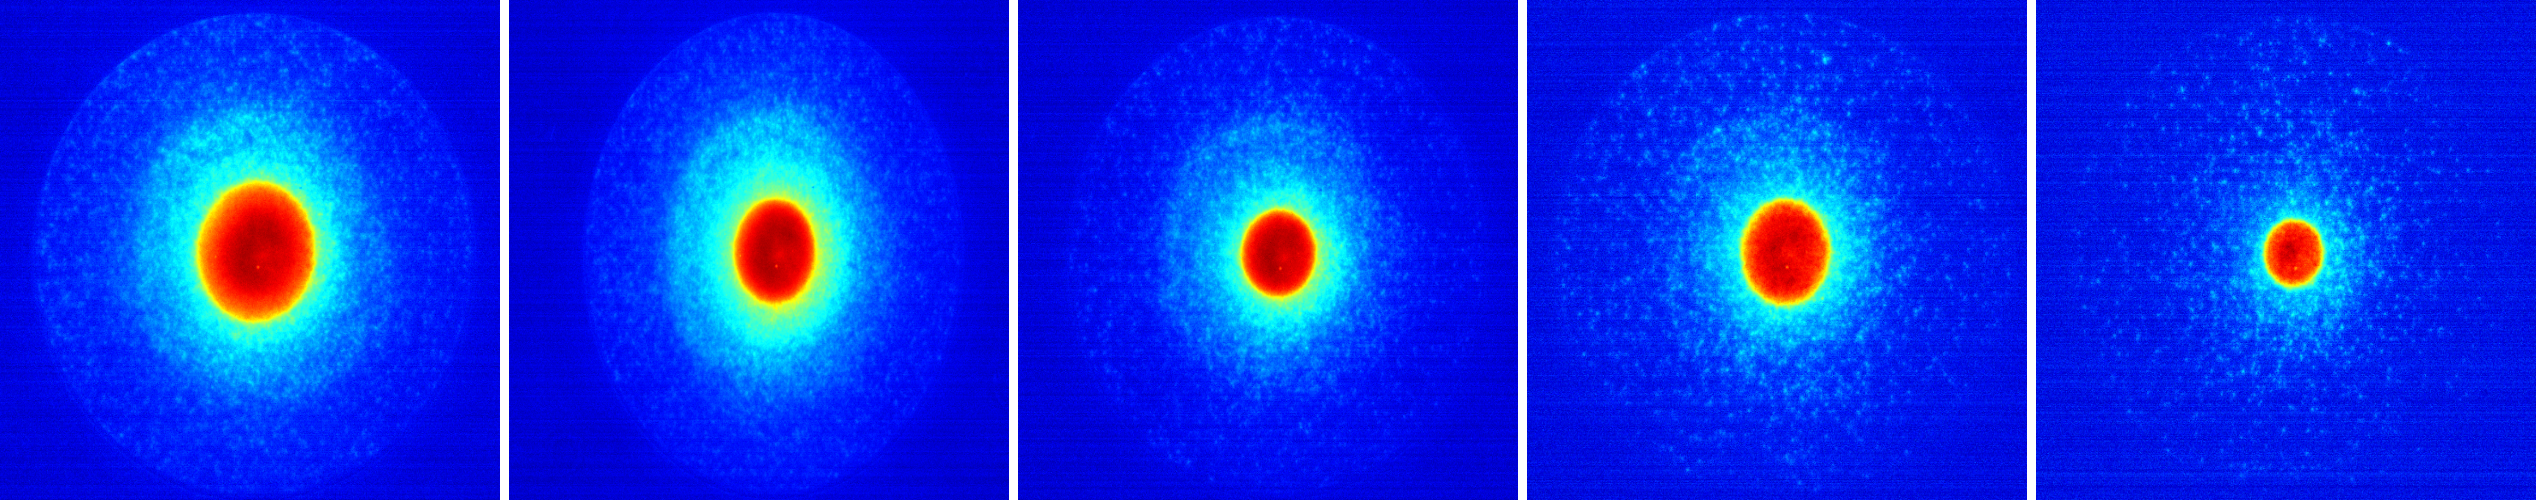
\includegraphics[width=1\textwidth]{../Images/results/NI_He_Dropletsize/RAW_NIR_HE_dropletsizeBigg.png}   				\end{subfigure}
\begin{subfigure}[l]{0.7\textwidth}
\caption{Typical VMI signal for small He droplets in NIR}
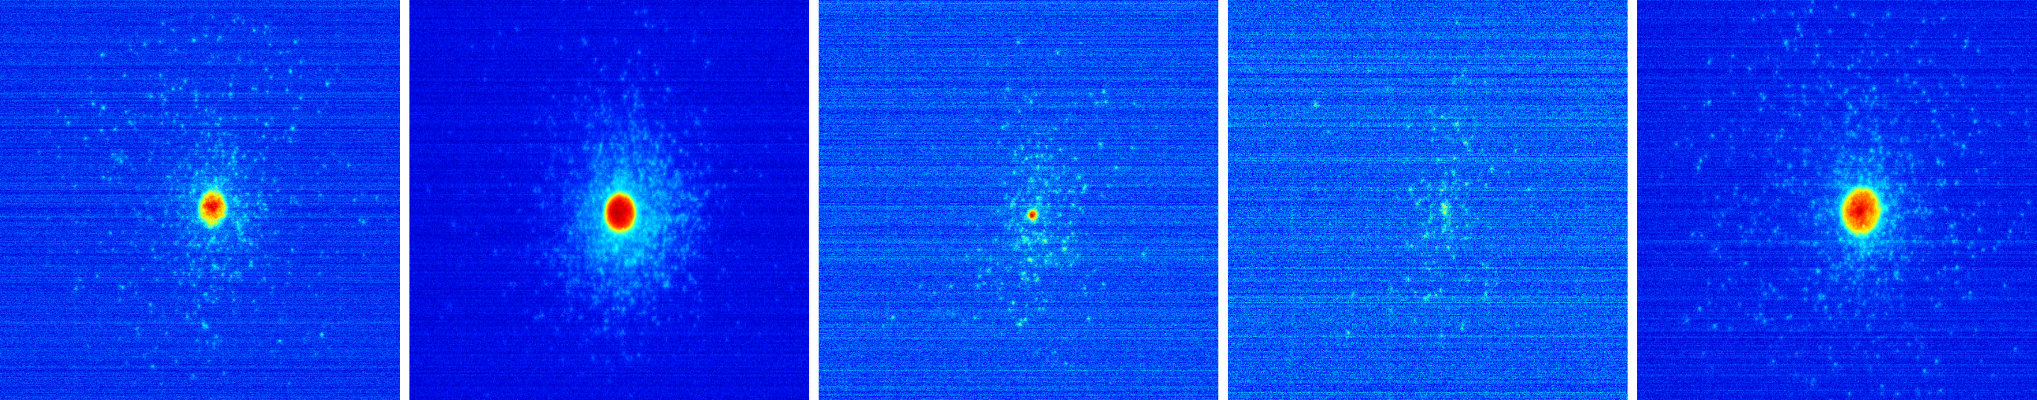
\includegraphics[width=1\textwidth]{../Images/results/NI_He_Dropletsize/RAW_NIR_HE_dropletsizeSmall.png} 
\end{subfigure}
\caption[MIR He droplet scan histograms]{On the left, The histogram for max energy and on right, the histogram for number of electrons.}
\label{fig:NIRsample}
\end{figure}

In the next sections, special attention will be taken on the VMI results due the amount of information it can deliver. The TOF data, is analyzed in an independent way, but will not be part of the main results. The data done in Heidelberg were already analyzed in the master thesis of Nicolas Rendler and the information can be found in \cite{rendler_einzelschuss_2017}. The main purpose to re-evaluate this information is to compare the experiments with similar parameters to the ones used in ELI-AlPS.

Fig. \label{fig:NIRsample}  show some example of the variety of radius and intensities in the He signal in NIR, it presents high and low intense signal for different experiments. On the top, the high brightness allows to see an outer circle, close to the frame of the pictures, that is the limit of the detector, the border of the MCP arrange. All signals present a similar behaviour,a uniform circular blob with a defined edge surrounded by a cloudy background. The most frequent signals are the small and less intense pictures like the bottom row, but as seen, high energetic explosion are reachable, specially in the bigger droplets as explained in the following sections. 

Fig. \ref{fig:NIrsummed} left, shows an example of hundreds of individual he signals summed and normalized, on the right it  inverse Abel transform PES done in Pbasex for different droplet size (Nozzle temperatures). The Energy distribution shows a clear trend independent of the nozzle temperature. It presents a first shoulder around 1 and 2 eV and decaying constantly down to 50eV taht is the maximun of the detector. It means that the summed signal has a sharp derivation on the intensities, showing that the average signal presents a defined maximal energy (radius) similar to the single  explosion signals, so from the next subsection  the data presented will be evaluate from the single shot explosion.

\begin{figure}[h!]
\centering
\begin{subfigure}[l]{0.4\textwidth}
\includegraphics[width=1\textwidth]{../Images/results/Comparison_energyDistribution/NIr_He_12K.png}   				\end{subfigure}
\begin{subfigure}[l]{0.59\textwidth}
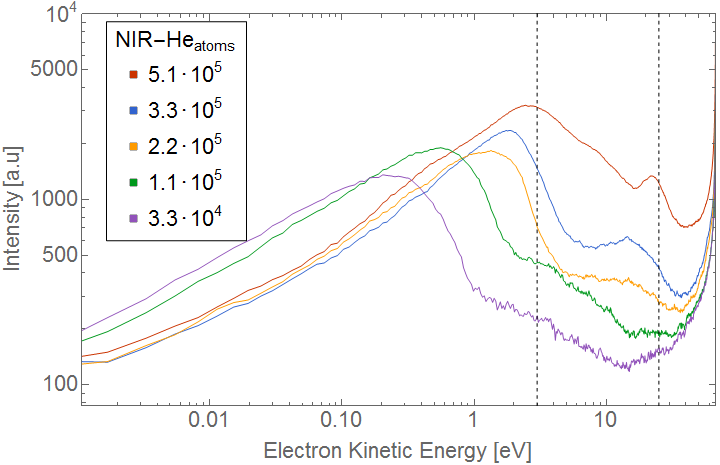
\includegraphics[width=1\textwidth]{../Images/results/Comparison_energyDistribution/NIR_He_summed_energydist.png} 
\end{subfigure}

\caption[MIR He droplet scan histograms]{On the left, The histogram for max energy and on right, the histogram for number of electrons.}
\label{fig:NIrsummed}
\end{figure}


\subsection{Laser Parameter Dependence}

Using the "Xenon ion charge" intensity calibration on the NIR laser we obtained table \ref{tab:nirintens}with the corresponding intensity at the focus depending on the power. The laser power was measured just before the beam enters to the detection chamber and was compared also to the theoretical calculations for the optical system mounted as shown in Fig. \ref{fig:xeionchargecalib}. In order to have the best results and high data acquisition, we worked at maximum intensity near $77$ mW to ensure a good quality of the ignition process and hence its efficiency.

\begin{table}[t]

\centering
\begin{tabular}{|l|c|}
\hline
\multicolumn{1}{|c|}{$Power{[}mW{]}$} & $Laser intensity {[}W/Cm^{2}{]}$ \\ \hline
11                                  & 6,27E13                                           \\ \hline
25                                  & 1,425E14                                          \\ \hline
55                                  & 3,135E14                                          \\ \hline
80                                  & 4,56E14                                           \\ \hline
115                                 & 6,555E14                                          \\ \hline
\end{tabular}
\caption[NIR laser power to intensities]{Laser focused intensities calculated for different Powers }
\label{tab:nirintens}
\end{table}


\begin{figure}[h!]
\centering
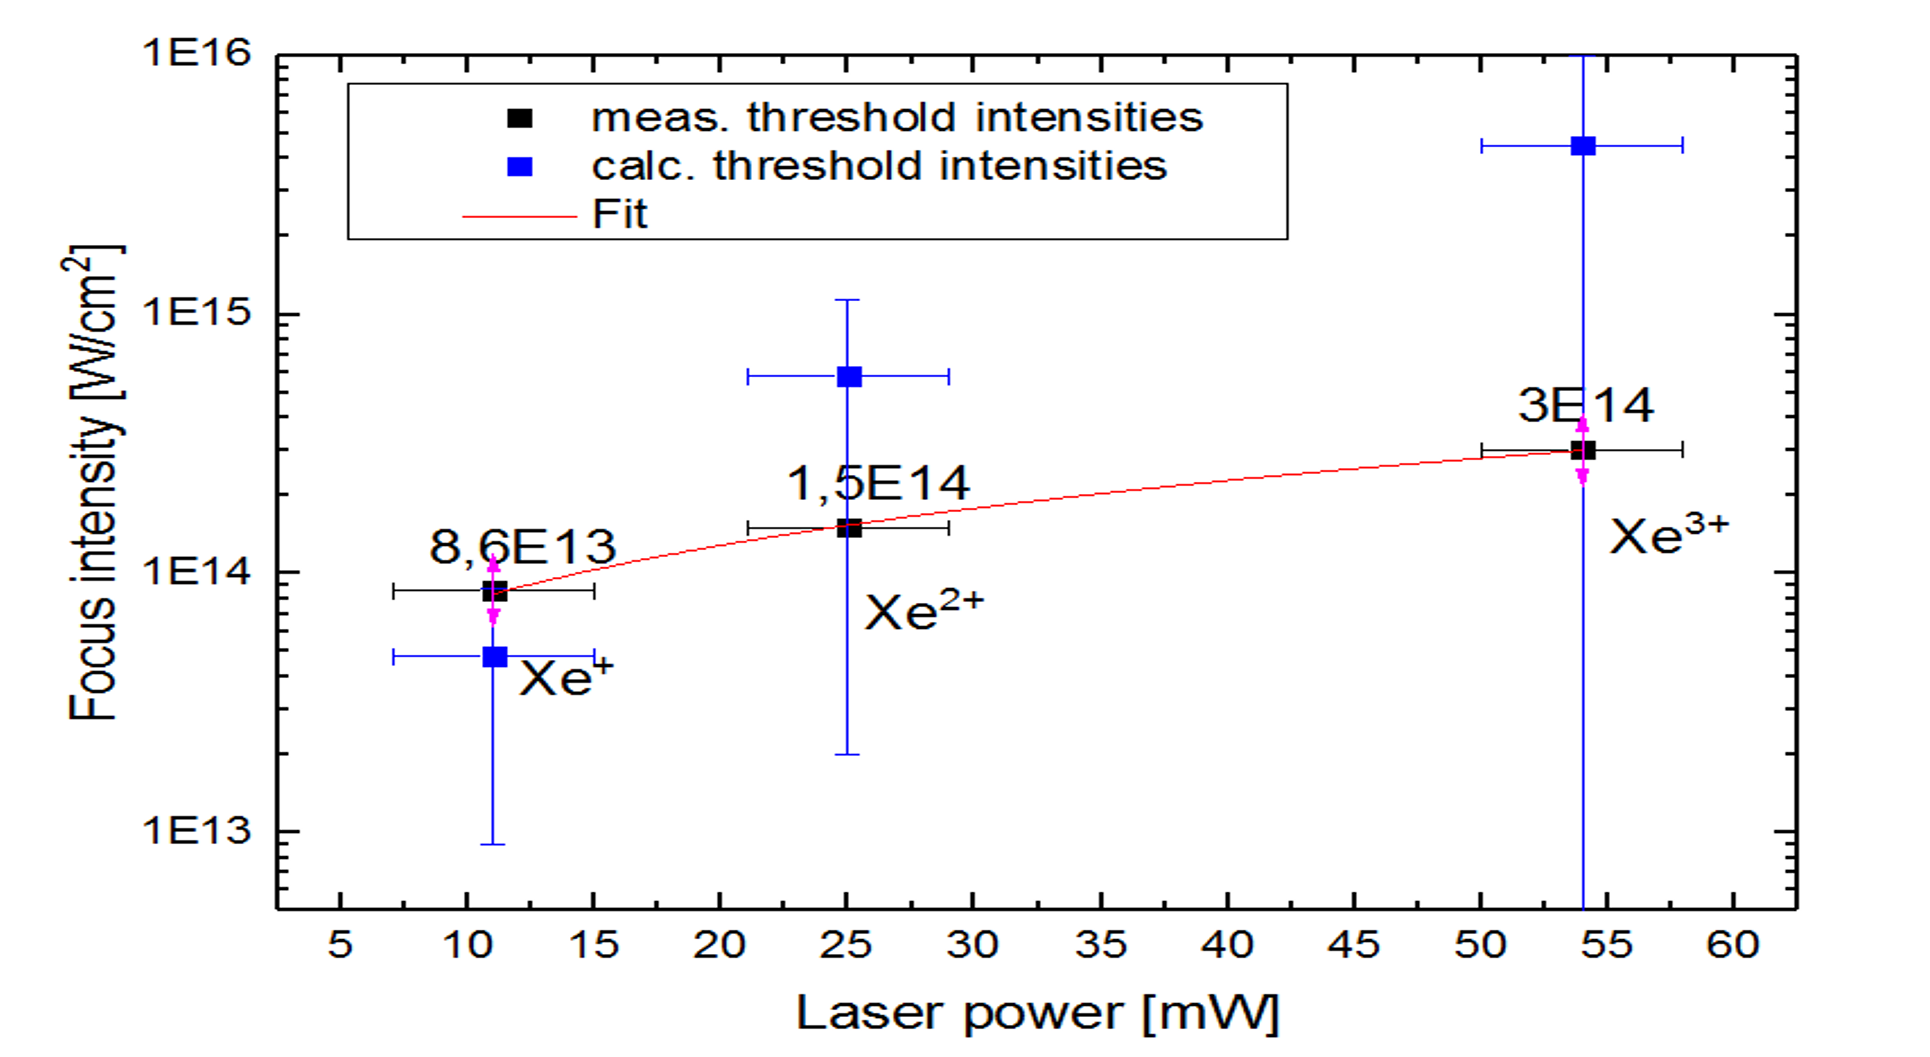
\includegraphics[width=10 cm]{../Images/Xeioncharges_intensitycalib.png} 
\caption[Xenon ion charge calibration for NIR] {Xenon ion charge calibration for NIR laser at three different power. On Blues the calculated threshold intensities and on black the experimental results for the power measured before the laser beam enter to the detection chamber.}
\label{fig:xeionchargecalib}
\end{figure}

\subsubsection{He Droplet  Intensity Dependence.}

The laser system used at the Max-Plank-Instituted is a NIR laser at $800nm$ wavelength and a rate of $10Hrz$ and a $d_{pulse}=23$ fs pulse duration. Helium clusters at the same nozzle temperature $T_{nozzle}=12.2$ K and  backing pressure of $P_{0}=45$ mbar were doped with Xenon at a fix doping level, with the a constant pressure measured in the oven chamber of $P_{oven}=2E-6$ mbar. This measurement were taken with a slightly smaller MCP-PHS arrangement of $d=42.2mm$ diameter of active area. At this nozzle temperature the Helium droplet have proximate $N=397390$ atoms before going through the oven chamber and its doped with $Xe_{dop}=134$ atoms, given a final number of He number of $N=386596$ atoms. The VMI voltages where set to VMIx2 and the MCP and PHS to $1250$ V and $4000$ V respectively. The camera was stablish to exposure time of $t_{exp}=1$ ms. 50000 pictures were taken for 7 different laser power, at $55,80,115,140,185,210$ and $240$ mW. 

\begin{figure}[h!]
\centering
\begin{subfigure}[l]{0.49\textwidth}
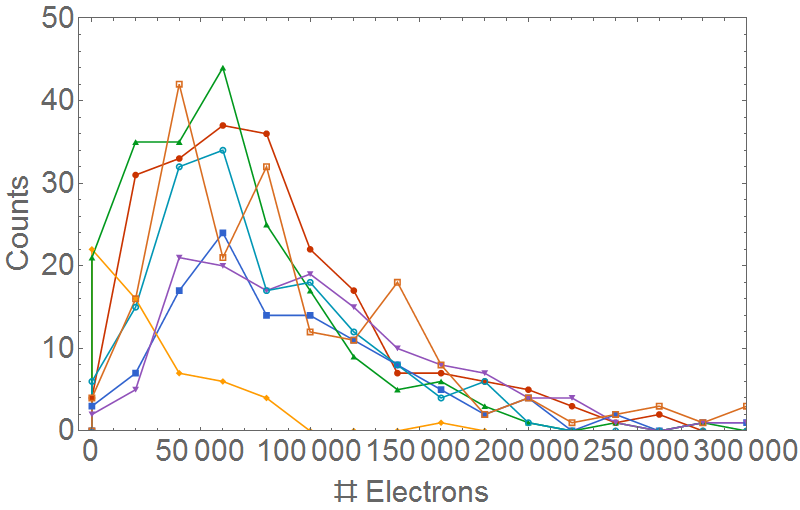
\includegraphics[width=1\textwidth]{../Images/results/NIR_He_intensityscan/Helec.png}   				\end{subfigure}
\begin{subfigure}[l]{0.49\textwidth}
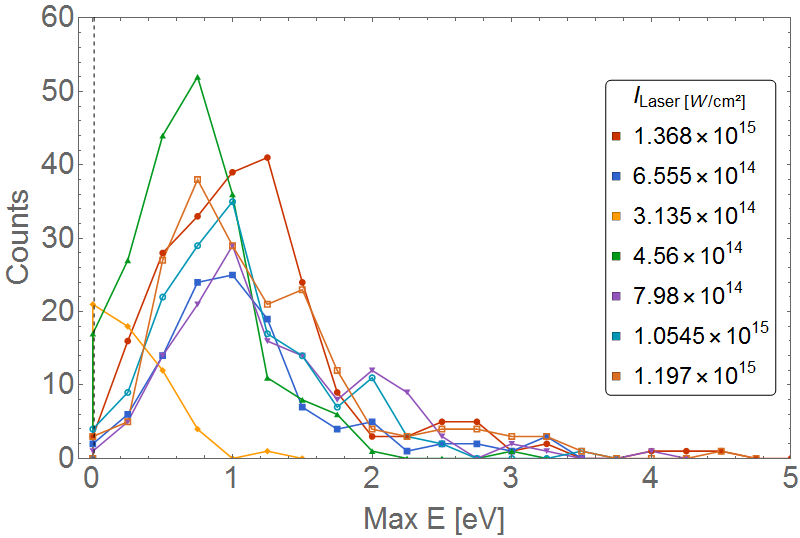
\includegraphics[width=1\textwidth]{../Images/results/NIR_He_intensityscan/Henerg.png} 
\end{subfigure}

\caption[NIR He Intensity dependence. Histograms]{On the left, The histogram for max energy and on right, the histogram for number of electrons.}
\label{fig:NIRHesummed}
\end{figure}

After the signal is detected, the blob finder protocol is used in order to determine the radius and brightness of each picture and transform it to  number of electrons and max energy. Fig \ref{fig:NIRHesummed} presents the histogram for the Number of electrons (Left) and the max energy (right) for the different laser intensities. As shown the histogram presents a clear distribution around 60000 electrons and 1 eV respectively. Both histograms present the shapes of a a Boltzmann distribution ramping up the values in the lower energies faster and electrons and a slower slope for the higher ones, where the higher the intensities the farther the location of the peak distribution. The dash line on the energy plot represents the minimun energy that the algorithm can detect. 

%%Despite the changing signal rate, we compare the Energy distribution depending on the number of electrons, a clear distribution on all signals is shown. In fig \ref{fig:NIRHEdistribution}, each blue point represents a individual picture, where the radius and brightness of each signal bloop is identified. Once all signal are analyzed, the distribution is plotted and fitted. The red line, is a fit based on $E_{max}= B \cdot n^{2/3}$, Eq. 3.12 where B is the B-Factor named on Eq. 3.13 and $n$ is the number of electrons, the $2/3$ factor is fix. The same process is done for each of the data sets at different laser intensities. All fits have the same tendency regardless the laser intensities, changing slightly on the B-factor. This in an important outcome meaning that the data fits quite well to our simple spherical electronic cloud model. As the B-factor is directly related to the density of the electronic cloud using Eq. 3.11 is possible to delimit the radii of the electronic sphere. In other words, according to this model, if we know the total number of electrons it’s possible to calculate the maximal energy that we can detect. 


Fig. \ref{fig:NIRHEall} top, shows that the signal rate depends strongly on the laser intensity, but even at lower intensities some coulomb explosion can be found. Although the percentage of pictures with signal decrease remarkably, we never find zero signal meaning that there is enough  initial ionization to start the coulomb explosion. Fig \ref{fig:NIRHEhistograms} bottom shows the mean number of electrons and the mean E$_{max}$, we see that them reach a maximum after $I=8.5E14$ W/cm$^{2}$ and keeps comparably constant for the following intensities. This result is not surprising because we don't expect large differences on the energies reached after the system is fully ignited, suggesting that after the beginning of the process, the coulomb explosion keeps a constant behaviour. First, the laser intensity play a fundamental role in given the starting condition to the nanoplasma formation but after a threshold, the laser does not influence in the final coulomb explosion any more. Second, a clear density limit is shown, it is possible that it is influence by this limitation of the laser on the process, but mostly it can be limited by the droplet size that was used in the experiment, as consequence, the biggest droplets are all expanding so in order to find bigger energy and densities we should use lower nozzle temperatures.  

 \begin{figure}[h!]
\centering
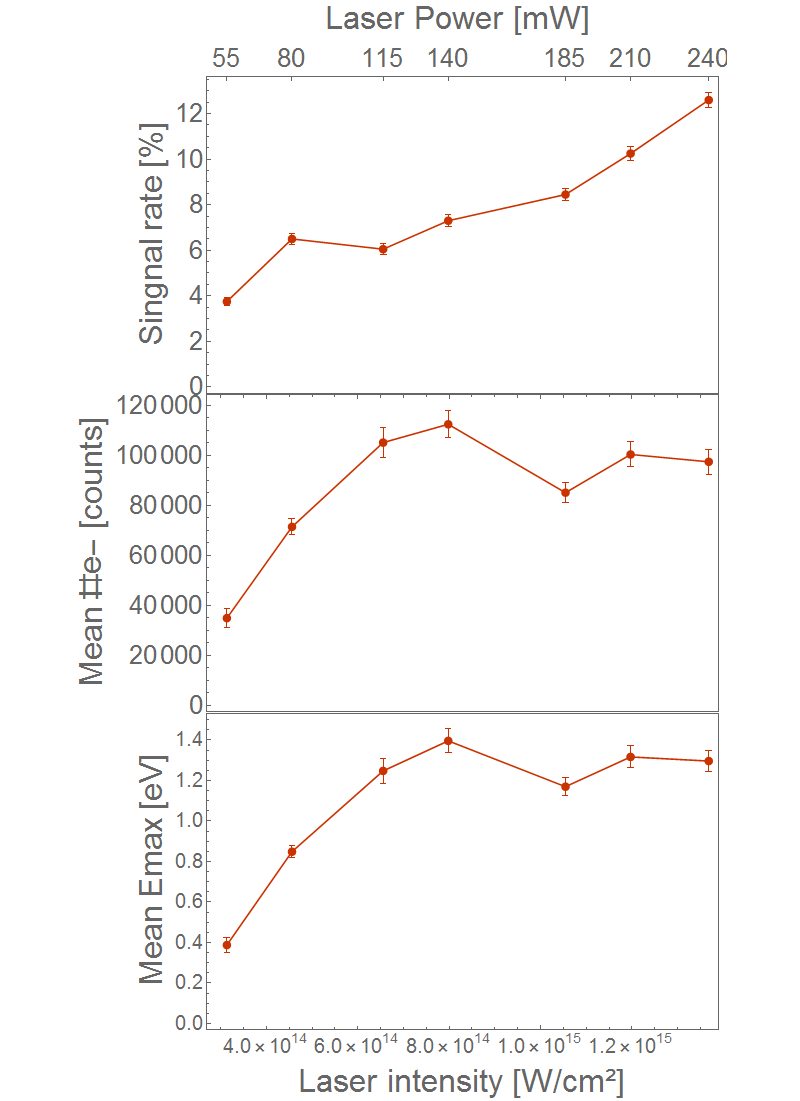
\includegraphics[width=0.5\textwidth]{../Images/results/NIR_He_intensityscan/Alltogether.png} 
\caption[NIR He intensity dependence. Signal Rate and Mean Values)]{On top, the signal rate at different laser intensities. On bottom,the Mean number of electron and the mean Max energy for the different laser power. The error bar correspond to the standard derivation for each data set.}
\label{fig:NIRHEall}
\end{figure}



\subsection{He Droplet size dependant.}

 For this data set, helium clusters at different nozzle temperatures, were doped with Xenon, with a doping pressure 2$E$-6 mbar measured in the doping chamber. The VMI were set to VMIx1 voltages and the MCP and PHS to 1250 V and 3400 V respectively. The camera was set to $\tau_{exp}=1$ ms exposure time. 50000 pictures were taken for 5 different temperatures, at 12.5 K, 13 K, 14 K, 16 K and 20 K. The data were analyzed using the data processing mentioned in chapter 3 to convert the bloop radius and its inner brightness to Maximal energy $E_{max}$ and Number of electrons $\#e-$.  Using the Hagena scale \cite{hagena_cluster_1972}, we can calculate a prediction of the total number of atoms before and after the doping. Table \ref{tab:NIRclustersize} shows the  mean number of atom per cluster to at the different nozzle temperatures and also its corresponding number of dopant. 

%\begin{table}
%\centering
%\begin{tabular}{|l|l|l|l|}
%\hline
%\multicolumn{4}{|c|}{NIR  Helium Cluster Size (Ref)}                            \\ \hline
%$T_{Nozzle} {[}K{]}$ &$ N_{He no dop}$ & $ N_{Xe atoms}$ & $N_{He}{[}atoms{]}$ \\ \hline
%20                    & 32671          & 66        & 27362                      \\ \hline
%16                    & 108424         & 199       & 92432                      \\ \hline
%14                    & 222264         & 189       & 207173                     \\ \hline
%13                    & 331040         & 149       & 319084                     \\ \hline
%12                    & 509035         & 160       & 495949                     \\ \hline
%\end{tabular}
%\caption[NIR  Helium Cluster Size]{NIR  Helium Cluster Size}
%\label{tab:NIRclustersize}
%\end{table}

\begin{figure}[h!]
\centering
\begin{subfigure}[l]{0.49\textwidth}
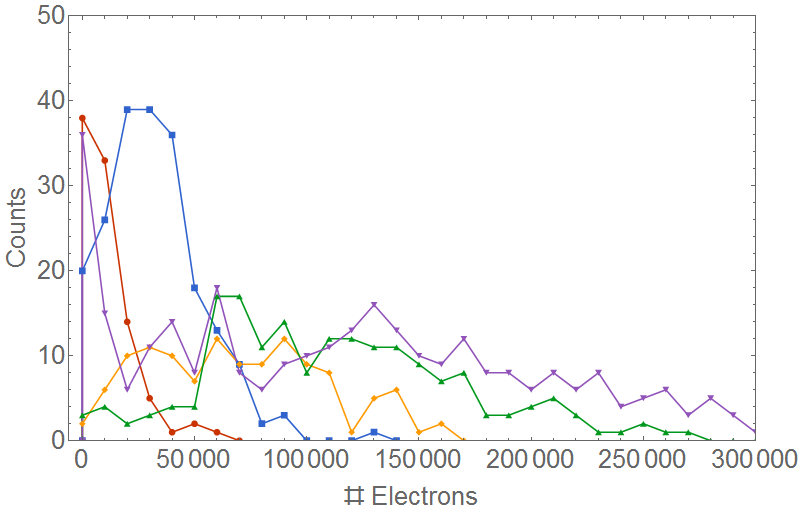
\includegraphics[width=1\textwidth]{../Images/results/NI_He_Dropletsize/HElectrones.png}   				\end{subfigure}
\begin{subfigure}[l]{0.49\textwidth}
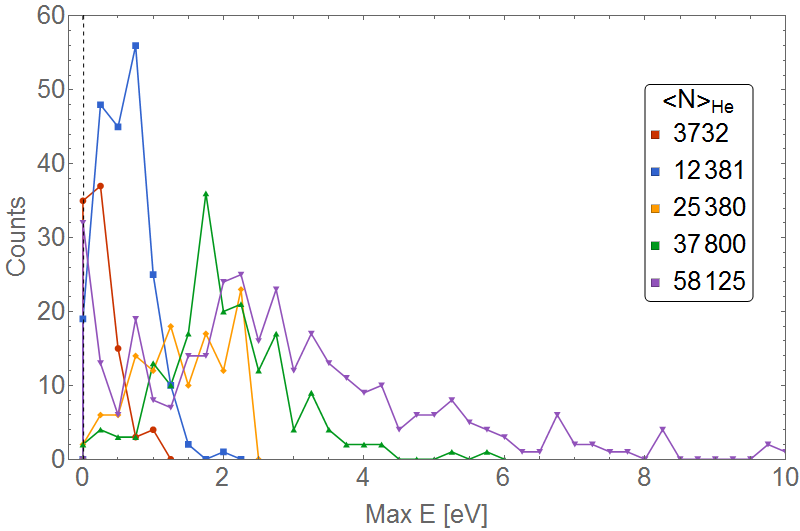
\includegraphics[width=1\textwidth]{../Images/results/NI_He_Dropletsize/HEnerg2.png} 
\end{subfigure}
\caption[NIR He droplet size. histograms]{On the left, The histogram for max energy and on right, the histogram for number of electrons.}
\label{fig:NIRHehistosize}
\end{figure}

Similar as the last subsection, radius and brightness of each signals were transform to max energy and number of electrons using the blob finding routine. Fig \ref{fig:NIRHehistosize} shows the histogram for the Number of electrons (left) and the max energy (right) for the different number of atoms  <N> in the cluster. The histogram presents contrasting distributions with stiff and clear peaks for the smaller droplets and broader dispersion for the bigger droplets. For the num of electrons, the smallest droplets have a peak lower than the 50000 while the lower nozzle temperatures have a plateau structure over 80000, same for the energies with peak in 1 eV and 2.5 eV respectively.

 \begin{figure}[h!]
\centering
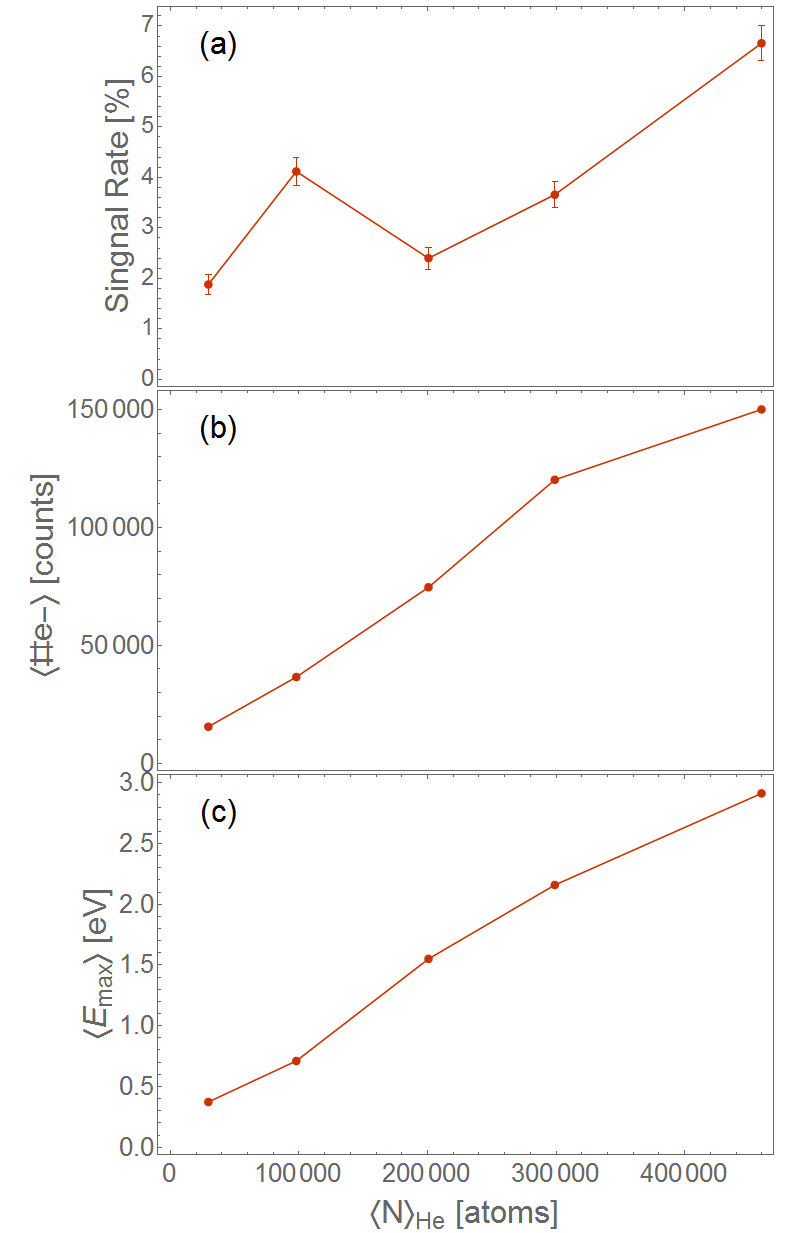
\includegraphics[width=0.5\textwidth]{../Images/results/NI_He_Dropletsize/Alltogether.png} 
\caption[NIR He intensity dependence. Signal Rate and Mean Values)]{On top, the signal rate at different laser intensities. On bottom,the Mean number of electron and the mean Max energy for the different laser power. The error bar correspond to the standard derivation for each data set.}
\label{fig:NIRHEall}
\end{figure}

Fig. \ref{fig:NIRsrEnergy} shows the corresponding signal rate depending on the nozzle temperature. As shown, the biggest droplets contain the highest percent of signal compared to the small droplets. We need to take into account that the difference in size helps to the ignition of the process due the cross section for the interaction with the laser field also increase, so the ionization is easy. Furthermore, the larger the number of atom in the cluster the most electrons available to be detected. In the Mean $\#$e- and E$_{max}$ values, for example at 12 K, the mean energy shows that exist counts for high energetic explosion, up to 4 eV, but the mean value of all the data is not higher than 3 eV. This behaviour is also present for the other nozzle temperatures, where there exist a broad distribution for 13, 14 and 12 k with mean values further from the biggest value.
Moreover, the number of electron in the system also rise with the size, for $T=$12.2 K the mean number is close to 150000 electrons, almost 10 time bigger than the smallest droplets, who is also 10 time smaller. Similar as in the signal rate, the mean values present a linear dependence with the droplet size. This trivial relation is due the increment on the number of electron available in the system, so the bigger the droplet the bigger the explosion. 

% Once identified the radius and brightness of all the pictures, a Energy distribution is plotted. Fig \ref{fig:NIRsrEnergy} right, shows the energy distribution for the droplets sizes at 12.2 K. Each blue point represented a single picture, with the bloop radius and brightness transformed to energy and electrons. The red line, is a fit based on Eq. 3.12 where B is the B-Factor named Eq. 3.13 and $n$ is the number of electrons, the $2/3$ factor is fix to the fitting. The same process is done for the other nozzle temperatures, the fits have the same tendency for different droplet sizes and don't deferrer much between each other. For the B-factor at 12.5 K the corresponding electronic cloud density is around $\rho =2.2 [1/\mu m^{3}]$, what leads to a electronic cloud radius of  4.3 $\mu$m. 

\section{Helium Nanoplasma in MIR Fields }
 
In this section helium nano droplets doped with different alkaloids are described. Helium was expanded from a nozzle of $5 \mu m$ opening at a backing pressure of $P_{0}=30 bar$, using different nozzle temperatures. This beam is doped with a xenon gas when passing through a gas doping cell in the doping chamber or Calcium atom when it pass through the oven. Therefore, the mean dopant cluster size is determined by the xenon pressure in of the gas doping cell, which is controlled by a high-precision needle valve and the oven temperature. The flight distance through the gas doping cell is $30mm$. The MIR laser pulses are orthogonal to the cluster beam through a vacuum window into the chamber and focused into the cluster beam by a focusing mirror.
The laser intensity in the focus during the measurements was in average $2.5E14$ W/cm$^{2}$ at a maximum power of $P\sim 10$ W , it had a minimum pulse duration of $t_{pulse}=45$ fs and a rate of 10 KHz. The laser power depends on the pulse duration because the total pulse energy needs to be distributed on time, in each specific case we will denote the power when it changes. The polarization of the laser field was orthogonal to the spectrometer axis. The electronic signals were recorded with the Basler CCD camera at a minimal exposure time $t_{Exp time}=45 \mu$s triggered with the TOF as explained in chapter 3, this process grants the single shot signal. The camera is focused on the MCP-PHS arrange that makes the electron signal visible. 

\begin{figure}[h!]
\centering
\begin{subfigure}[l]{0.7\textwidth}
\caption{Typical signal for small He droplets in MIR}
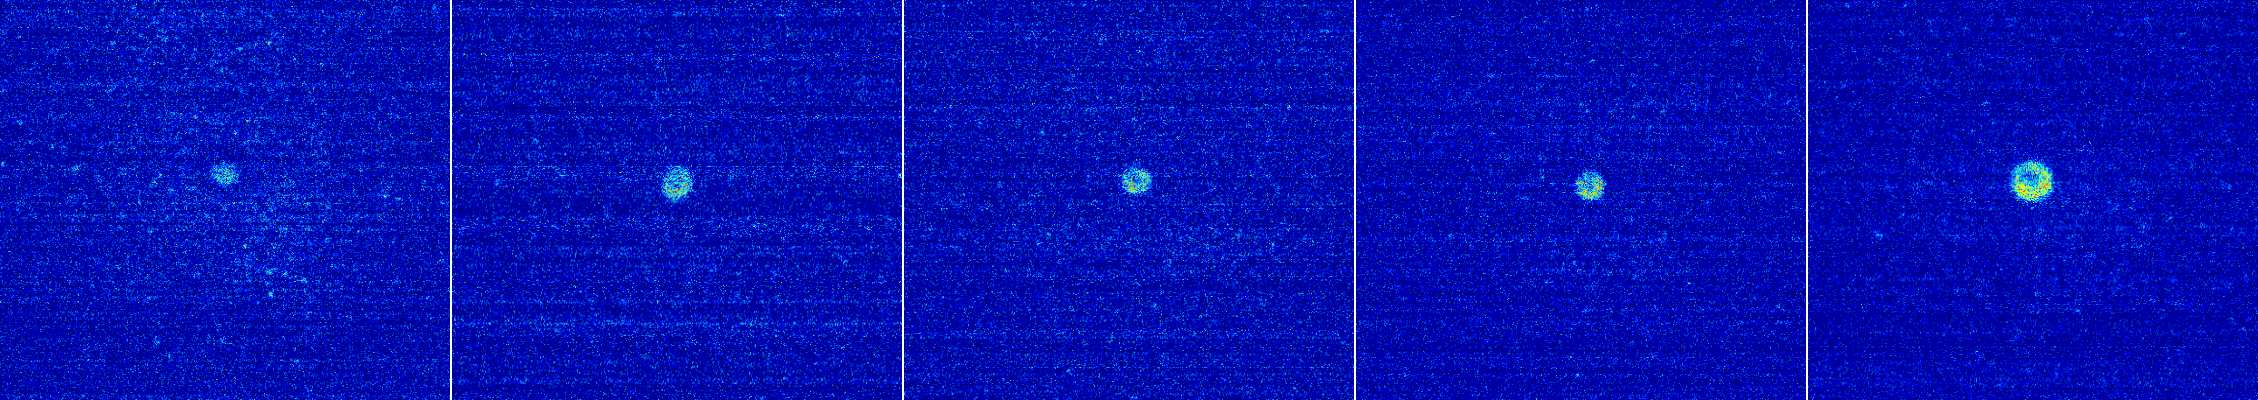
\includegraphics[width=1\textwidth]{../Images/results/Mir_He_Dropletsize/RAW_MIR_He_smalldroplets.png}   				\end{subfigure}
\begin{subfigure}[l]{0.7\textwidth}
\caption{Typical signal for big He droplets in MIR}
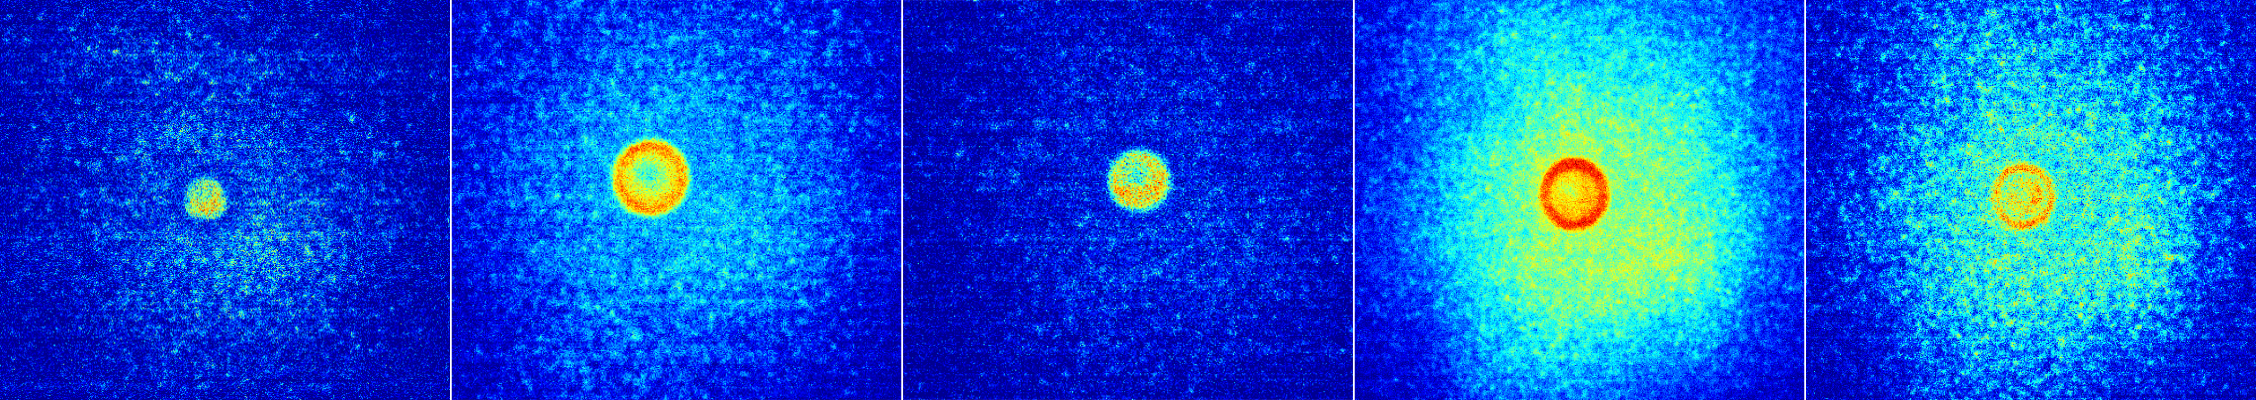
\includegraphics[width=1\textwidth]{../Images/results/Mir_He_Dropletsize/RAW_MIR_He_bigdroplets.png} 
\end{subfigure}

\caption[MIR He raw images]{On the top, the typical pictures for small He droplets explosion of low intense signal. On the bottom, the typical pictures for the big He droplets that usually contains the more intense signals. Also, the donut shape is present in either some of the small signals as in the bigger ones}
\label{fig:MIRHeexample}
\end{figure}

We do not expect that all laser shot hits a cluster or generates a plasma explosion, so  most of the data sets presents low signal rate, in order to have representative statistics, in each experiment were taken 10000 pictures, about less than $10\%$ had signal. Fig\ref{fig:MIRHeexample} shows  example of different range of explosions and signals. Most of the VMI signal had the expected circular aspect except for the larger size droplets, with the donut shape. Because we are using a bigger MCP, we cut the images closer to the center avoiding analyze irrelevant data.

Fig. \ref{fig:MIRHeenergdist} left, shows an example of hundreds of individual he signals summed and normalized at 10.5 K, on the right it inverse Abel transform PES done in Pbasex for different droplet size. As before, the energy distribution shows a clear trend independent of the nozzle temperature. It presents a first shoulder around 0.1 eV and decaying constantly down to 12 eV. It decrease fast until 1 eV what means that the summed signal has a sharp change on the intensities, showing that the average signal presents a defined maximal energy (radius) similar to the single  explosions as well.

\begin{figure}[h!]
\centering
\begin{subfigure}[l]{0.4\textwidth}
\includegraphics[width=1\textwidth]{../Images/results/Comparison_energyDistribution/MIr_He_10K5.png}   				\end{subfigure}
\begin{subfigure}[l]{0.59\textwidth}
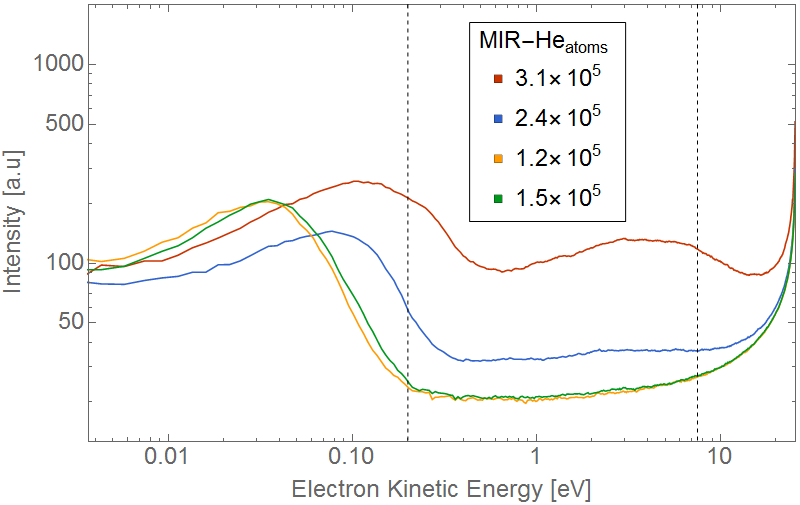
\includegraphics[width=1\textwidth]{../Images/results/Comparison_energyDistribution/MIR_He_summed_energydist.png} 
\end{subfigure}

\caption[MIR He droplet scan histograms]{On the left, The histogram for max energy and on right, the histogram for number of electrons.}
\label{fig:MIRHeenergdist}
\end{figure}

\subsection{Helium Droplet Size Dependence.}

For this data set, He clusters at different nozzle temperatures, were doped with Xenon at a pressure of $0.0060$ mbar measured in the gas doping cell. The voltages were set to VMIx1  and the MCP and PHS to $1600$ V and $4000$ V respectively. The camera was set to minimum exposure time and the trigger system was used. 100000 pictures were taken for 4 different temperatures, at 10.6 K, 11 K, 12 K and 12.5 K. The data where evaluated once more as last section, demonstrating that the Trigger system worked efficiently. As result, it was shown that even for this high repetition laser rate, single shot signals can be achieved. The TOF signal work as a reference to identify the single explosion, and then each individual VMI picture is treated as follows. Fig \ref{fig:tofhe} shows a mean TOF for the measurement at 10.6 K. As we can see, there is a large amount of water and a small peak for hydrogen still in the vacuum chamber, this remain gases affect especially for the background. It is shown that Helium is effectively ionized due the peak at He$^{+}$ but on contrast no He$^{2+}$ signal was identify.

\begin{figure}[hbtp]
\centering
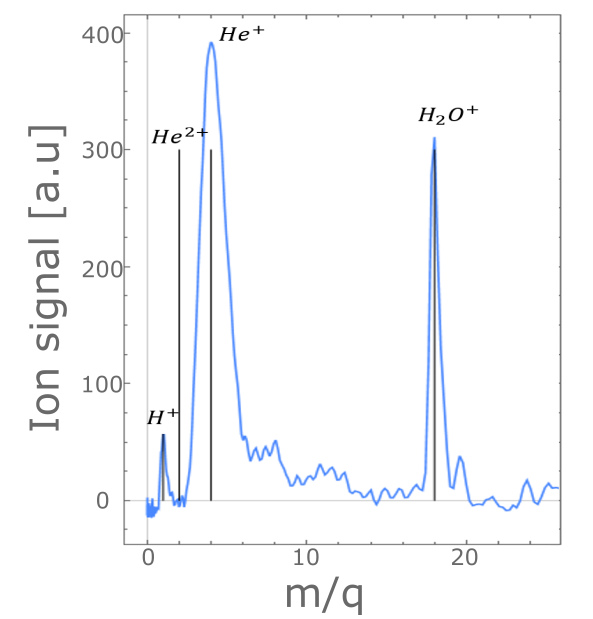
\includegraphics[width=0.5\textwidth]{../Images/results/Mir_He_Dropletsize/tof.png}
\caption[MIR TOF spectra He ]{Mean TOF spectra for He at 10.6 K. The }
\label{fig:tofhe}
\end{figure}

Using the experimental data taken on the NIR experiments by Nicolas Rendler \cite{rendler_einzelschuss_2017}, we can extrapolate the data to have a prediction of the total number of atoms before and after the doping. Table \ref{tab:clustersize} shows the mean number of atom per cluster to at different nozzle temperatures and also its corresponding number of dopants. As reference for the cluster size scaling, we used data at $P_{0}=50$ bar and temperatures similar to the experiment. 

\begin{table}[t]
\centering
\begin{tabular}{|l|l|l|}\hline
\multicolumn{3}{|c|}{Cluster Size reference}                                                             \\\hline
T$_{Nozzle}$ {[}K{]}  & N$_{Xe atoms}$ & $\langle$N$\rangle$ $_{He atoms}$ \\ \hline
10.6                  & 220     & 2.80$\cdot$10$^{5}$                      \\ \hline
11                    & 192     & 2.29$\cdot$10$^{5}$                       \\ \hline
12                    & 138     & 1.42$\cdot$10$^{5}$                      \\ \hline
12.5                  & 119     & 1.13$\cdot$10$^{5}$                    \\ \hline
\end{tabular}
\caption{cluster size reference}
\label{tab:clustersize}
\end{table}


%\begin{figure}[h!]
%\centering
%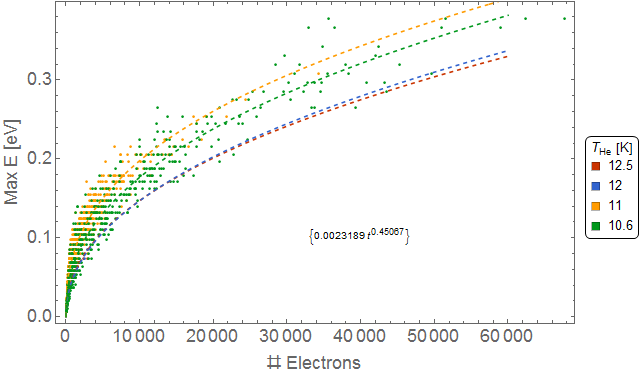
\includegraphics[width=0.5\textwidth]{../Images/results/Mir_He_Dropletsize/fits.png} 
%\caption[He-Xe droplet size distribution]{Maximal Energy distribution on the number of electrons. On colors the different nozzle temperatures, the smallest droplets (12 K,12.5K) presents few signal images and can be seen behind the yellow and green  points in the left-bottom of the graphic.  The dash line are the fit curves.}
%\label{fig:energdistributionHeXeSize}
%\end{figure}
%
%%Fig \ref{fig:energdistributionHeXeSize} shows the energy distribution versus the number of electrons. As we can see, most of the data point lay on the bottom-left of the graph at lower energies, but the distribution also show signals with energies up to 0.4 eV and 50000 electrons collected, this signals comes from the most energetic coulomb explosions, and we can clearly see that the bigger the droplet the  brightness we can get. Due the few signal for the 2 higher temperature we discard the 2 fit lines, moreover, for the others, its fit lines are in a relatively good concordance to the data using Eq. 3,13 as a guide, we find a B-factor $B=0.00305103$ and a factor $k=2/5$. 

%On one hand, the first big different with the experiments with the NIR laser, is this non correlation to the uniformly charged Cloud model, especially in the exponent $k$, that changes from 1/3 to 2/5. There is no theoretical background that can predict this behaviour but as the exponent is closely linked to the geometry of the cloud, we can assume the fits does not agree because the  big droplets are not perfectly spherical, so for example, as they are liquid, the droplets could turn in an ellipsoidal. This new exponent is persistent in all the fit for the MIR experiments in helium. On the other hand, as explained, the B-factor is directly related to the density and in consequence to the radius of the electronic cloud. Given B, we obtain approximately $R_{cloud}=85$  $\mu$m, a radius three order of magnitude bigger that the initial cluster, that for example at 11 K have $R_{cluster}=13$ nm.

The MIR and NIR signals present large similarities except for the high intense pictures with a localized energy on the edge, a ring shape with low brightness in the center and a high intensity in the edge of the blobs. Despite this differences, it does not affect the signal analysis due we are based on the max energy and not in the internal distribution. Fig \ref{fig:histodropletsize} shows the histogram of the $E_{max}$ and  $\#$e- for the different temperature. On one hand, in the $E_{max}$, the first peaks describe that most of the droplets achieve energies between $0.05$ and $0.1$ eV, decreasing rapidly after that. On contrary, the biggest droplets have a more broaden distribution that the higher temperatures. Furthermore in the $\#e-$, a broader distribution is show, a huge density is found for droplets with less than 2000 electrons, having a drastic decrease. It show a clearly distribution where the main average size of the droplet is small,  but without discarding that some individual points at a huge number up to 80000 $e-$.

\begin{figure}[h!]
\centering
\begin{subfigure}[l]{0.49\textwidth}
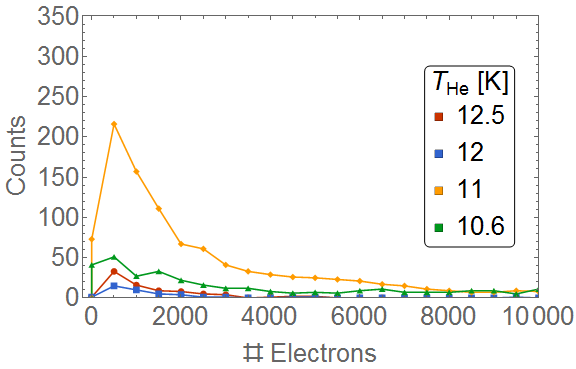
\includegraphics[width=1\textwidth]{../Images/results/Mir_He_Dropletsize/Helec.png} 
\end{subfigure}
\begin{subfigure}[l]{0.49\textwidth}
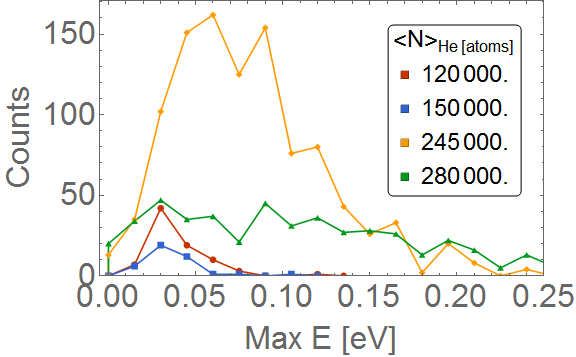
\includegraphics[width=1\textwidth]{../Images/results/Mir_He_Dropletsize/Henerg.png}   				\end{subfigure}
\caption[MIR He droplet scan histograms]{On the left, The histogram for max energy and on right, the histogram for number of electrons.}
\label{fig:histodropletsize}
\end{figure}

Fig \ref{fig:Alldropletsize} presents the Signal rate and the Mean values for the number of electrons and max energy depending on the temperature of the nozzle. As shown the figure, for the biggest droplet (points to the right) we got the largest signal rate at 10.6 K and 11 K and immediately for the smaller droplet the rate decrease drastically, same tendency is show in the mean values, making clear that plasma is easier to ignite at lower temperatures. Therefore, as more electrons and energy are detected while the signal rate increase, we assume that the nanoplasma formation is more efficient for larger droplets. The drop on the signal rate at 10.6 K compared to the 11 K can evidence a loss of efficiency for the laser to ionized even bigger droplets. In other words, After certain droplet size, is more difficult to ignite the plasma.  Unfortunately, no other measurement where taken at lower temperature to confirm if this is a statistical event or a real effect.

\begin{figure}[h!]
\centering
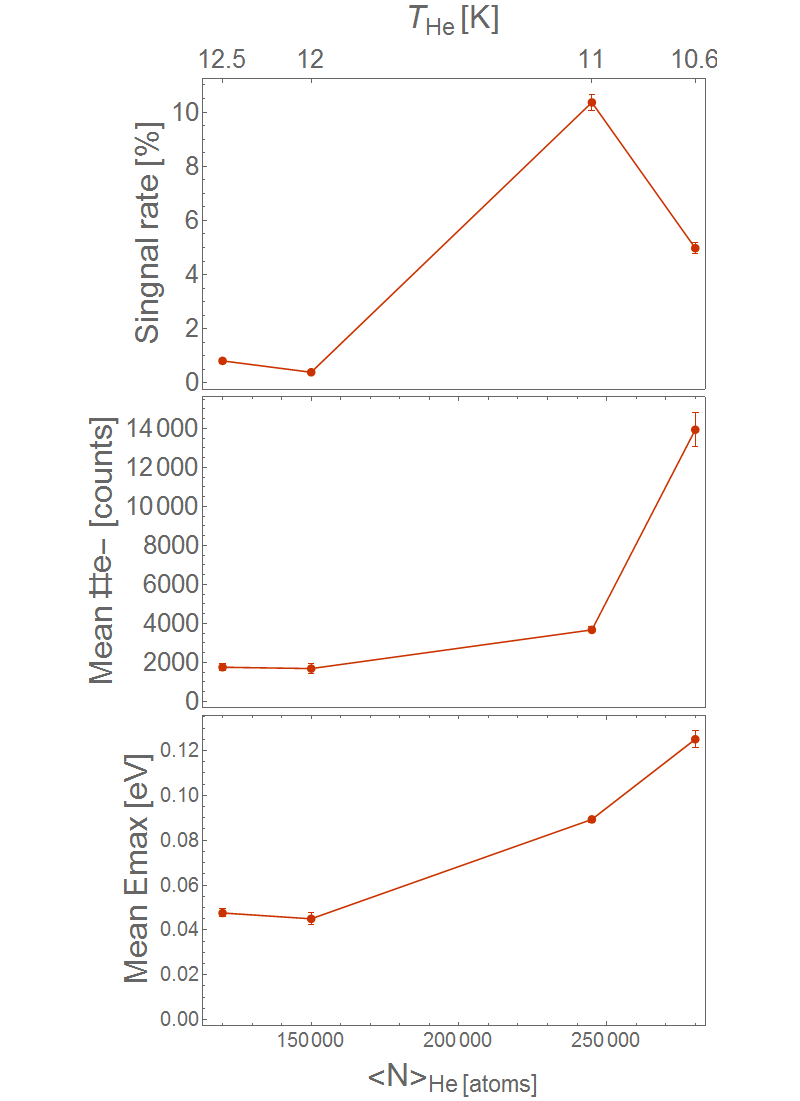
\includegraphics[width=0.5\textwidth]{../Images/results/Mir_He_Dropletsize/Alltogether.png} 
\caption[MIR He droplet size dependence]{On top,the signal rate in percentage of the pictures with signal depending on the nozzle temperature. On bottom, the mean of the number of electrons and the Max energy for each point respectively.}
\label{fig:Alldropletsize}
\end{figure}

\subsection{Doping Dependence}

One of the advantages of the setup is the possibility to exchange easyly the doping element. Here we present the results of four different dopants at different level in He droplets. Xe and Ar were introduce trougth the needle valve to the doping cell while the calcium was evaporated from the oven. Fig \ref{fig:He-dopingexample} present typical examples of the signal at each doping element. Although the signal varies in intensity, specially for the Ar doping, the  shape and structure looks similar to the above experiments, so same procedure will be apply.

\begin{figure}[h!]
\centering
\includegraphics[width=0.6\textwidth]{../Images/results/MIR_He_XeCaDop/RAW_MIR_He_alldoping.png} 
\caption[MIR HeDoping examples]{typical signals for He cluster doped with Ar, water, Xe and a Xe-Ca mixture. The signal varies in intensity, on top the usual low brightness and on bottom the more intense pictures}
\label{fig:He-dopingexample}
\end{figure}

\subsubsection{Helium-Argon Doping.}

In this data set, He clusters were doped with Argon at different gas doping pressures. Helium was produced at a nozzle temperature $T_{nozzle}= 11$ K and ignited by the MIR laser pulse, the VMI were set to VMIx1 voltages and the MCP and PHS to 1700 V and 4000 V respectively. The camera was set to $t_{exp}$=50 $\mu$s exposure time what means the data was not correlated with the same trigger. The exposure time was modified due the low signal rate, nevertheless the information will be still evaluate in the same way  as before, taking into account that signal rate was so low that is possible to have single shot.  100000 pictures were taken for 3 different doping pressures, at $2E-4, 6E-4$ and $12E-4$ mbar measured in the gas doping cell. 

\begin{figure}[h!]
\centering
\begin{subfigure}[l]{0.49\textwidth}
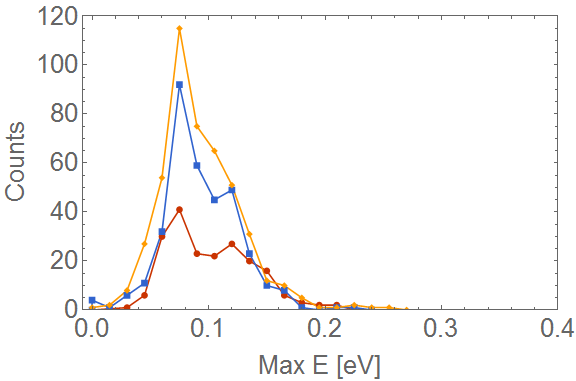
\includegraphics[width=1\textwidth]{../Images/results/MIR_He_ArDop/Henerg2.png} 
\end{subfigure}
\begin{subfigure}[l]{0.49\textwidth}
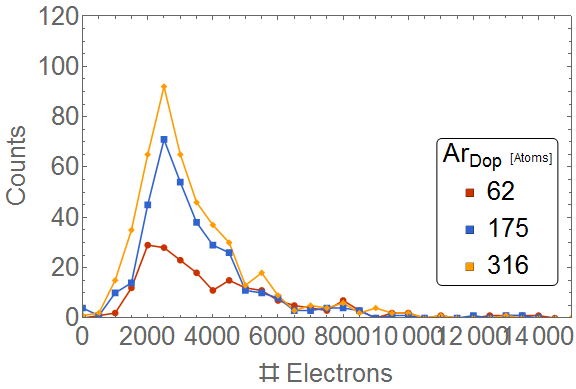
\includegraphics[width=1\textwidth]{../Images/results/MIR_He_ArDop/Helec.png}   				\end{subfigure}
\caption[MIR He_Ar. Histograms]{On the left, The histogram for max energy and on right, the histogram for number of electrons for He clusters in MIR laser at different doping level.}
\label{fig:histoArdop}
\end{figure}

Fig \ref{fig:histoArdop} shows the histogram for the He droplts doped with Ar at different doping levels, On the lefth the max energy distibution shows peaks around 0.1 eV with a similar distribution independent the doping level, Same in the mean number of electrons (left), where the peak is paround 3000 e- and the disposal of the plot shows similar tendency

%Fig \ref{fig:HeArEnergydistr} shows the maximal energy distribution for three different pressures and it corresponding number of dopant. As mentioned, the signal rate for this data set was quite low showing that the efficiency for this doping is lower than for Xe. In red the fit done with the same fitting parameters than above with a B factor $B=0.09714$ what gives us a mean radius for the electronic cloud of  $R_{cloud}=$92.4 $\mu$m, quite proximately in the same order of magnitude to the data set above. For the Exponent, it was set as a free parameter given in general $k=2/5$ as well. 

As shown in the previous examples, the signal intensity for argon was low and it is reflected in Fig \ref{fig:He-Armean} where the signal rate (top) is lower that 5 $\%$. Here the amount of dopant increase the efficiency of the plasma, going from a 2 $\%$ up to 4.5 $\%$. Combined to the Mean values results, where the mean values decease with the doping, we can deduce that the efficiency for small droplets ignition also improves. As seen before,the histograms have a slightly broader distribution with high doping level, evidencing that the dopant helps in the plasma formation of the smallest droplets.
 
\begin{figure}[h!]
\centering
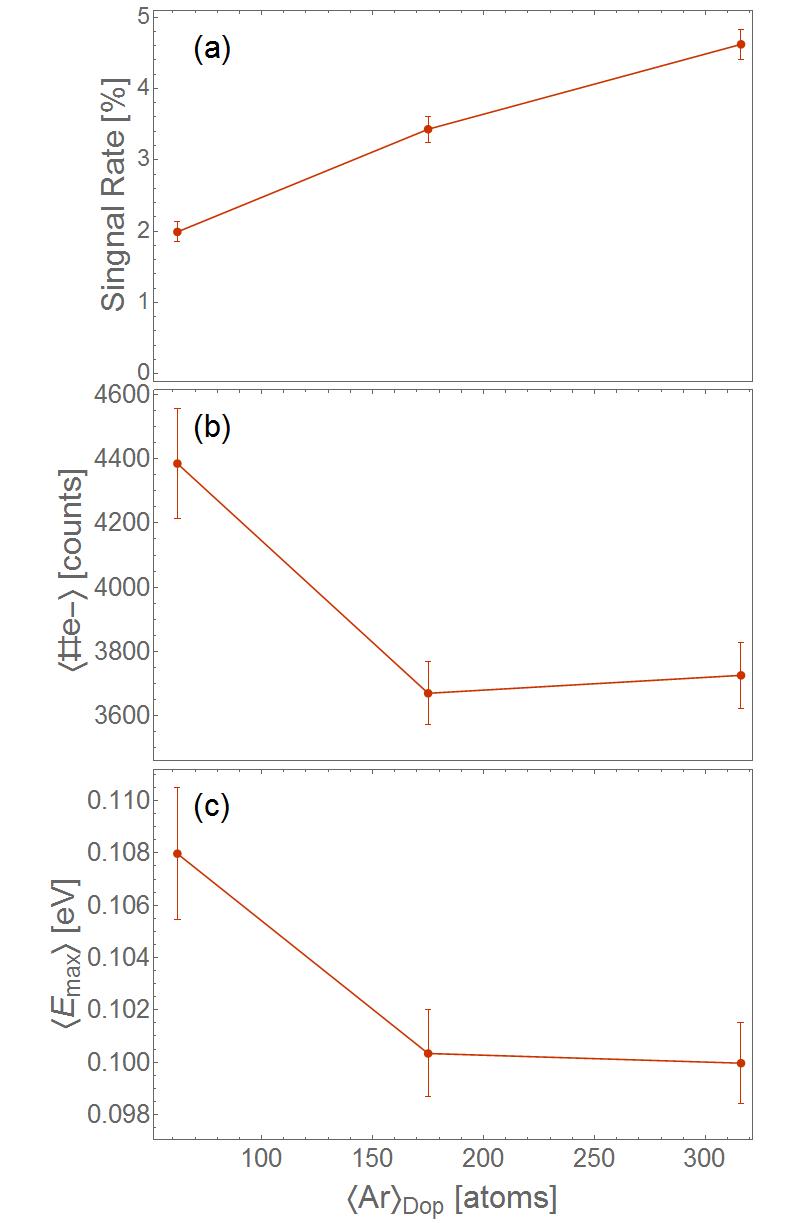
\includegraphics[width=0.5\textwidth]{../Images/results/MIR_He_ArDop/Alltogether.png} 
\caption[MIR He-Ar doping, signal rate and mean values]{On the top, the signal rate for the He-Ar doping. Center and bottom, are the mean values for the number of electrons and max energy respectively}
\label{fig:He-Armean}
\end{figure}

\subsubsection{Helium-Water Doping.}

One of the most commune and available dopants is water, not just because it is easy to get in the lab but also because it is also difficult to remove from the vacuum chamber. Even in our best vacuum, experiments usually contained few traces of water. In addition, at Mid-Infrared, water have a special resonance that could be advantageous because it will withstand a faster ionization and in consequence, a better creation of the plasma. This data set was taken with He droplets at $T_{nozzel}=11$ K doped with water. A small drop of water were located into the entrance of the needle valve, to achieve a controlled doping. The pressure at the gas doping cell was varied in order to perform several doping levels. The camera was set to $t_{exp}=120$ ms so single shot was not enable. The voltages were set to VMIx1 and the MCP and PHS to $1750$ V and $4000$ V respectively. 100000 pictures were taken for 5 different doping pressures, at 1$E-$4, 2$E-$4, 3$E-$4, 6$E-$4 and 12.5$E-$4 mbar. 

\begin{figure}[h!]
\centering
\begin{subfigure}[l]{0.49\textwidth}
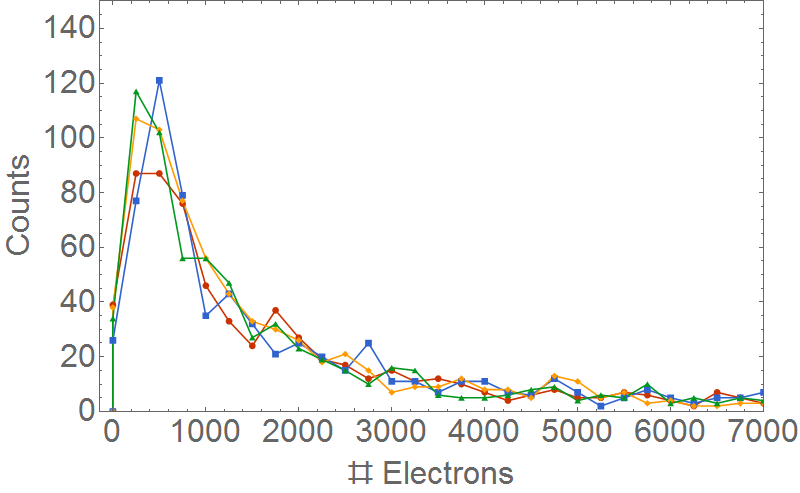
\includegraphics[width=1\textwidth]{../Images/results/MIR_He_waterDop/Helec.png} 
\end{subfigure}
\begin{subfigure}[l]{0.49\textwidth}
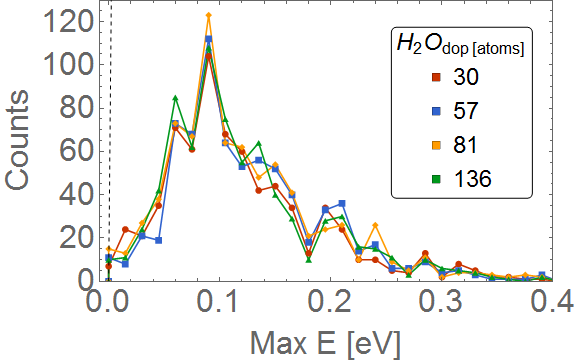
\includegraphics[width=1\textwidth]{../Images/results/MIR_He_waterDop/Heberg.png}   				\end{subfigure}
\caption[MIR He_Water. Histograms]{On the left, The histogram for max energy and on right, the histogram for number of electrons for He clusters with water in MIR laser at different doping levels.}
\label{fig:histowaterdop}
\end{figure}

Similar to the histograms above, fig \ref{fig:histowaterdop} presents small changes on the max energy distribution and number of electrons, where there is a well defined peak around 1000 e- and 0.1 eV. In this case the energy distribution does not present any broadening and the counts behaves independent on the doping level. The dash line in the left, represent the minimum energy (radius) that the blob finder can achieve.

%Fig. \ref{fig:He-waterEnergydistrib} shows the energy distribution for just one of water pressures. On blue are the points that represent the E$_{max}$ and $\#e-$ for an single signal picture and on red the fit based on the Eq. 3.12. For the water doping pressures the distribution looks almost the same, just changing in general the signal rate as shown in Fig. \ref{fig:Hewaterhistograms}. The fit function is used to find the B factor, obtaining for this example $B=0.01509$, that gives a radii for the electron cloud of $R_{cloud}=92.4 \mu$m, with an exponent factor $k=2/5$. 


Fig \ref{fig:He-Watermean} presents the signal rates and the Mean number of electrons and max energy depending on the water level. As shown, the three rates have similar and constant values, for the signal rate, the values oscillate around 7 $\%$ independent the doping level, On contrast to Argon. Same happens to the mean values that are around 3000 e- and 0.13 eV respectively.
As we showed, under the correct doping levels and He cluster sized, water molecules are a great dopant to ignite the He cluster in MIR laser pulses. The nanoplasma reach high energy states as well as a huge radius for the electronic cloud, reaching mean of electrons detected up to 70000. The mean values in the energy or electrons does not depend on the doping, as already described in the other experiments, once the ionization process ignites the plasma  the final result does not present variations.

\begin{figure}[h!]
\centering
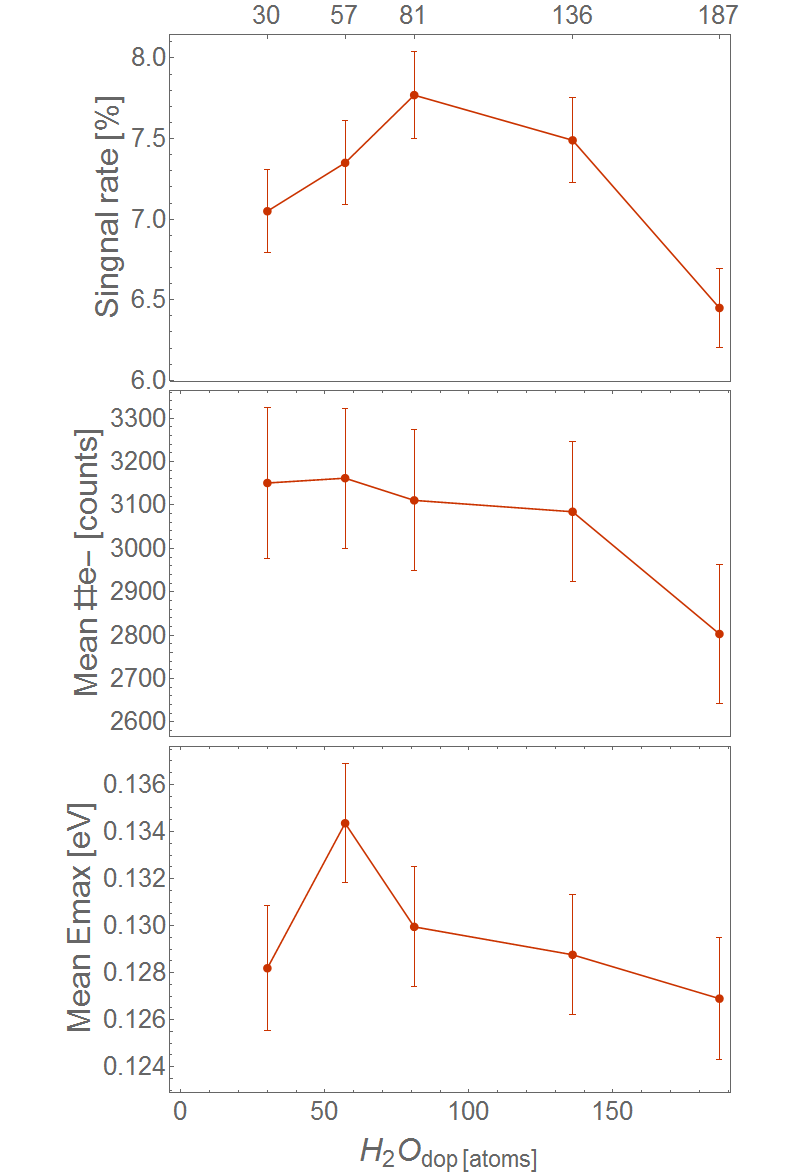
\includegraphics[width=0.5\textwidth]{../Images/results/MIR_He_waterDop/Alltogether.png} 
\caption[MIR He-Water doping, signal rate and mean values]{On the top, the signal rate for the He-Water doping at different doping levels. On the center and bottom, are the mean values for the number of electrons and max energy respectively}
\label{fig:He-Watermean}
\end{figure}

\subsubsection{Helium-Xenon-Calcium Doping}

In this experiment Helium clusters where doped with Xenon and Calcium atoms simultaneously. The Helium clusters were created at the same nozzle temperature $T_{nozzle}=10.6$ K and  a backing pressure of $P_{0}=30$ mbar. Xenon were introduce at 5 different pressures measured in the gas doping cell and Calcium was evaporated in the oven at 7 different temperatures. Table \ref{tab:dopXeCa} shows the sorted parameters used and their associate cluster size. The cells in the index (up and left) represent the number of atom for the Xenon and calcium for each data set while the inner cell shows their correlates mean He cluster size in atoms, The spaces in black are data set that were not taken.
The VMI voltages were set to VMIx1 and the MCP and PHS to $1600$V and $4000$V respectively. The camera was stablish to exposure time of $t_{exp}=34 \mu$s and single shot was assure. The laser power was monitored constantly to guarantee an average power of 10.7 W at pulses duration around $45$ fs.

\begin{table}[]
\label{tab:dopXeCa}
\centering
\begin{tabular}{|l|l|c|l|l|l|}
\hline
\backslashbox{Ca$_{dop}$}{Xe$_{dop}$} & \multicolumn{1}{c|}{0 atoms} & 30 & 90 & 180 & 350 \\ \hline
5 atoms & 2.4$\cdot$10$^{5}$ & 2.3$\cdot$10$^{5}$ & 2.3$\cdot$10$^{5}$ &  &  \\ \hline
7 & 2.3$\cdot$10$^{5}$ & \multicolumn{1}{l|}{2.3$\cdot$10$^{5}$} & 2.3$\cdot$10$^{5}$ &  &  \\ \hline
15 & 2.2$\cdot$10$^{5}$ & 2.2$\cdot$10$^{5}$ & 2.1$\cdot$10$^{5}$ &  &  \\ \hline
22 & 2.1$\cdot$10$^{5}$ & 2.1$\cdot$10$^{5}$ & 2.0$\cdot$10$^{5}$ &  &  \\ \hline
31 & 1.9$\cdot$10$^{5}$ &  & 1.8$\cdot$10$^{5}$ & 1.8$\cdot$10$^{5}$& 1.7$\cdot$10$^{5}$ \\ \hline
45 & 1.7$\cdot$10$^{5}$ & \multicolumn{1}{l|}{} & 1.6$\cdot$10$^{5}$ & 1.5$\cdot$10$^{5}$ &  \\ \hline
62 & 1.3$\cdot$10$^{5}$ & \multicolumn{1}{l|}{} & 1.3$\cdot$10$^{5}$ & 1.2$\cdot$10$^{5}$ & <N>$_{He_{atoms}}$ \\ \hline
\end{tabular}
\end{table}

\begin{figure}[h!]
\centering
\begin{subfigure}[l]{0.49\textwidth}
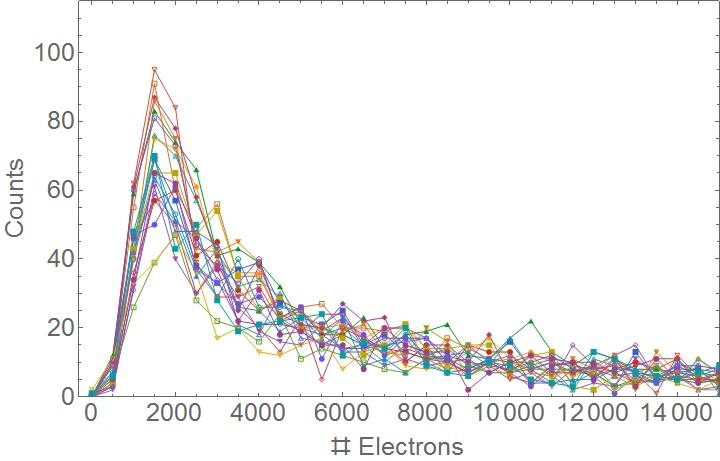
\includegraphics[width=1\textwidth]{../Images/results/MIR_He_XeCaDop/histoElectr.png} 
\end{subfigure}
\begin{subfigure}[l]{0.49\textwidth}
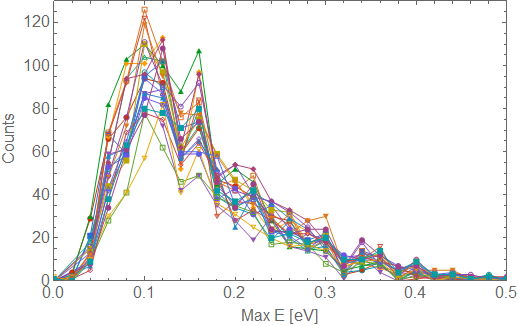
\includegraphics[width=1\textwidth]{../Images/results/MIR_He_XeCaDop/histoEnerg.png}   				\end{subfigure}
\caption[MIR He-Xe-Ca doping. Histogram]{On The left, the histogram for the Number of electrons for all doping levels. On the right, the histogram for the Max energies. The electron histogram was binned every 1000 e- while the energy was binned every 0.03 eV. The behaviours of the histograms follows the Boltzmann distribution and remains independently from the doping level, the counts remains  relatively constant.}
\label{fig:XeCahisto}
\end{figure}

In Fig\label{ref:XeCahisto} we present the histograms for $\#$e- and E$_{max}$. All the different doping are plotted in the same diagram in order to show that it doping the tendency does not change radically. As usual, the points are the individual pictures blob analysed and binned, the dash on the energy histogram represents the minimun energy that the finder can achive at 6 pixels. Further, the histograms we can show that the E$_{max}$ distribution is similar for all doping.  There is a defined peak close to 0.1 eV with a Boltzmann distribution likewise and a slow slop up to 0.4 eV. Moreover, the number of electrons present a peak close to 2000 with the slop decreasing down to 8000 where the counts reduce below 10. A second result to take into account, mentioned in the past section, is that the histogram share a peak electrons but the counts are reduce because of the signal rate as expected, so the dopant level does not play a big role in  the final distribution of the nanoplasma energy, but as we will see next, it does act in the signal rate and mean values.

\begin{figure}[h!]
\centering
\begin{subfigure}[l]{0.5\textwidth}
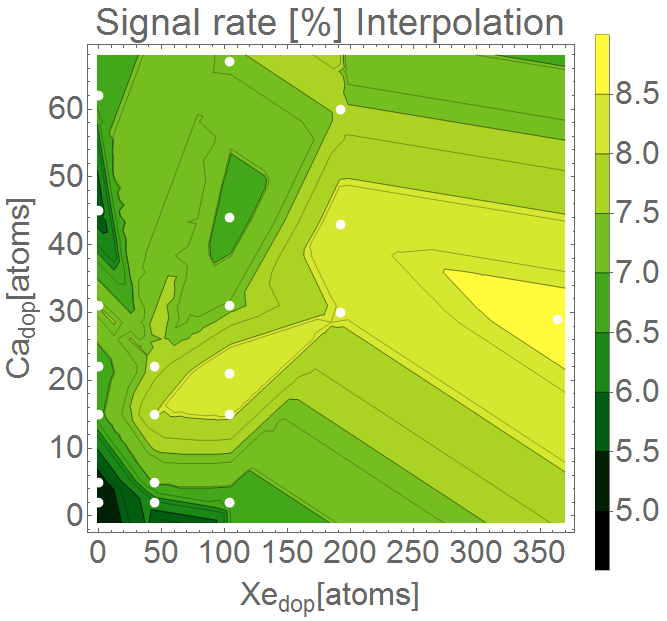
\includegraphics[width=1\textwidth]{../Images/results/MIR_He_XeCaDop/interpolationSignalRate2.png} 
\end{subfigure}\hfill


\begin{subfigure}[l]{0.49\textwidth}
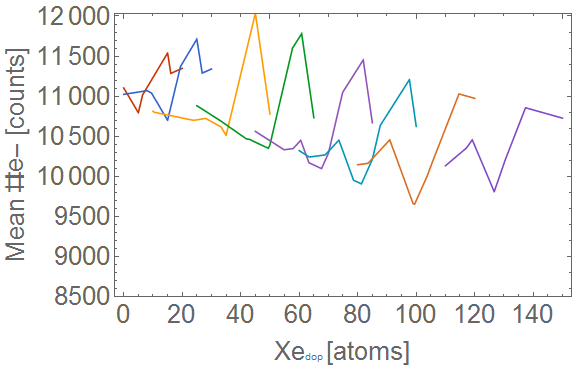
\includegraphics[width=1\textwidth]{../Images/results/MIR_He_XeCaDop/interpolationE2.png}   		
\end{subfigure}
\begin{subfigure}[l]{0.49\textwidth}
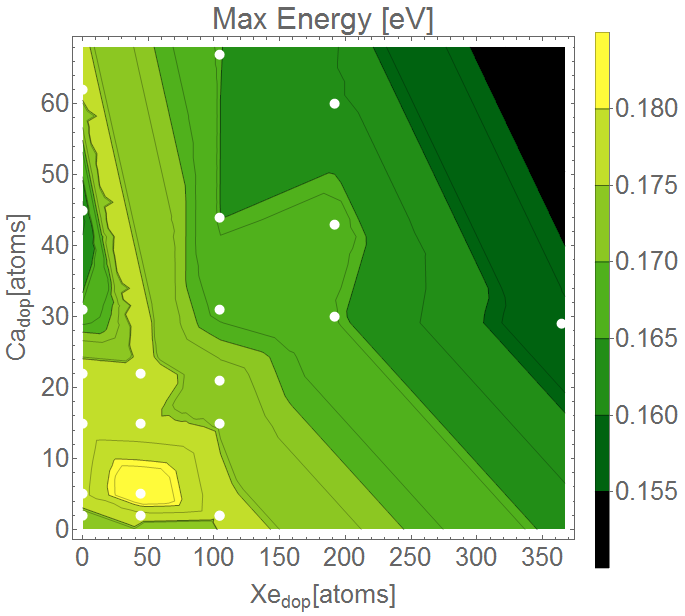
\includegraphics[width=1\textwidth]{../Images/results/MIR_He_XeCaDop/interpolationMax2.png}   	
	\end{subfigure}
\caption[MIR He-Xe-Ca doping. Interpolations]{From left to right, the interpolation for the signal rate in percentage, mean number of electron in counts and mean max energy in eV respectively. The green scale shows the intensity of the signal where the light yellow means high counts and the darker green lower counts. The white points represents the doping levels where the measurements were taken.}
\label{fig:XeCainterpolation}
\end{figure}

Fig \ref{fig:XeCainterpolation} shows an interpolation for the signal rate and mean values for the max energy and number of electrons. The green scale shows the signal intensity in percentage, $\#$e- counts and  energy in eV for each doping level respectively, on the bottom axis  the number of Xenon atoms and on the left axis the number of calcium atoms. The white points represent the doping levels where the measurement were done. According to the signal rate, there exist two maxima, one at Xe$_{100}$-Ca$_{20}$ and at Xe$_{360}$-Ca$_{30}$. The fist one is the most important because it shows an increment in the efficiency of the plasma formation at low doping comparable with the second peak where the number of dopants is 4 times longer. The histograms for electrons and energy also show a maxima but at low doping . The interpolation for the number of electron(center) presents the maxima at Xe$_{50}$-Ca$_{7}$ and a small depletion at  Xe$_{100}$-Ca$_{20}$ with a constant decrease for higher doping level. In contrast, the energy interpolation have the same maxima as the num of electron but does not present the depletion. Moreover, after the highest energy is present  a slow drop starts at  heavier Xe doping. At larger number of dopant the interpolation is less precise due the lack of measurement, nevertheless we can see that  for smaller droplets at heavy doping the cluster starts to deform and deplete it so the nanoplasma explosion is  less powerful.



%The dashed color line are cuts at a constant dopant numbers, for different constant  Xe+Ca at $40,50,65,85,100,120$ and $150$ atoms. The lines were choose in order that each line lay between 3 data points, so the interpolation could be accurate enough. On the right of fig \ref{fig:HeXECA-signalrate}, the cuts are plotted depending on the Xe atoms. This means that the right side of each line represent the doping with the maximum Xe atoms at the Xe+Ca constant,  once we go from right to left, we replace each Xe atom for one  Ca atom until we replace all Xe atom. Each line have a maximum of 40 points, because it was the max Ca doping measured. 

%
%An important result can de derive from Fig \ref{fig:HeXECA-signalrate}, as shown in the cut lines at constant total doping, we found a increment in the signal as the Ca doping replace the Xe. In all line, from right to left, the signal rate goes up when a few atoms of Ca are added despite the amount of Xe. It demonstrate a better efficiency in the doping for Xe-Ca combination compared to only Xe or only Ca. This tendency can be spot not just on the big crest in the interpolation between 70 to 120 Xe atoms and 15 to 25 Ca atoms, but also in each of the cuts, where the peaks are clearly display and the signal rate increase faster for these extra Ca atoms added, but once we reach a saturation maxima, the extra Ca atoms added makes the signal rate again decrees but in a slower way in most of the cases. 


%The same interpolation  was done for the histograms for the  number of electrons and maximum energy, Fig \ref{fig:HeXECA-NUmEle} and Fig. \ref{fig:HeXECA-Emax} shows the interpolation and cuts for constant dopant respectively. Fig \ref{fig:HeXECA-NUmEle} show one clear peak at low doping where the maximum  number of electrons appears, then for higher doping the counts starts to decreases and even a small depletion is shown in the range of Xe=100 Ca=20 atoms. On the right, the cut at constant dopant is show, the color from left to right represent the same cut done in the corresponding interpolation, and it’s necessary to read it at the same way. Where the right side of each line represents just Xe doping and each number to the left mean replacing one Xe atom for one Ca atom. As show, the exist also a recurrent peak efficiency in the nanoplasma ignition, meaning that at this peak the larger cluster are ionized, similar as shown on the Pulse duration scan. 


%Equally important. In the E$_{max}$ interpolation, a clear peak is also shown at Xe= 50 and Ca=7 atom,  This can be found in interpolation cuts, where the highly doped lines have a more constant performance and no real change is shown, but once we get close to the optimum doping (Yellow line), the replacement of Xe atom for Ca atoms becomes drastic effective, with a peak  founded close to 0.2 eV.  This measurement can be compare directly to the water doping scan where we show that once the ignition of the cluster starts, adding more water atoms does not creates changes in the process. Here, Xe doping results in a similar behavior, the points with just Xe atoms (Right edge of each colored line) have a relative constant mean energy, but once we introduce the Ca, dynamics start to appears, given a peak close to the Mean electrons interpolation. For the heavily doped clusters, on the blue, orange and purple cuts in the right, we see that the peaks are not present any more due the cluster destruction when to many atoms are added.

%
%If we compare the three interpolation, in a similar way we have analyzed the histogram in the last sections, we notice that the signal rate have a peak close to Xe=100 and Ca=20, but the Mean number of electrons and energy appears at lower doping. This means that at the most efficient rate, we are not igniting the biggest droplets but on contrary, they are being exploded closer to the zero doping.
\subsection{Laser parameter Dependence}

Similar to the experiments done in Heidelberg with the NIR laser pulse. We perform the experiments through different intensities and pulse duration in order to see the effects of the laser system on the coulomb explosion. The laser system used at ELI-Alps is at $3200$ nm wavelength and a rate of $100$ KHz.  One of the advantage of the laser system in ELI-Alps, is the possibility have a tunable pulse duration from $\tau_{pulse}=45$ ps to 250 fs.

Fig \ref{fig;MIrlaserraw} show some examples of raw VMI pictures at different pulse duration and in consecuence intensities. All signal conserve the same structure seens until now, a circle in the center of the detector with a clear edge that can be identified by our blop detector algorithm. One difference to the images in NIR is the intensity of the signal. Here the pictures are faint and  diffiult to recognize sometimes specially for the lowest intensity as we will show next.

\begin{figure}[hbtp]
\caption[MIR He laser parameter examples ]{Raw images for different pulse durations and laser intensities. The most of the pictures show low intensity signal, the donut shape is also present for some of them.}
\centering
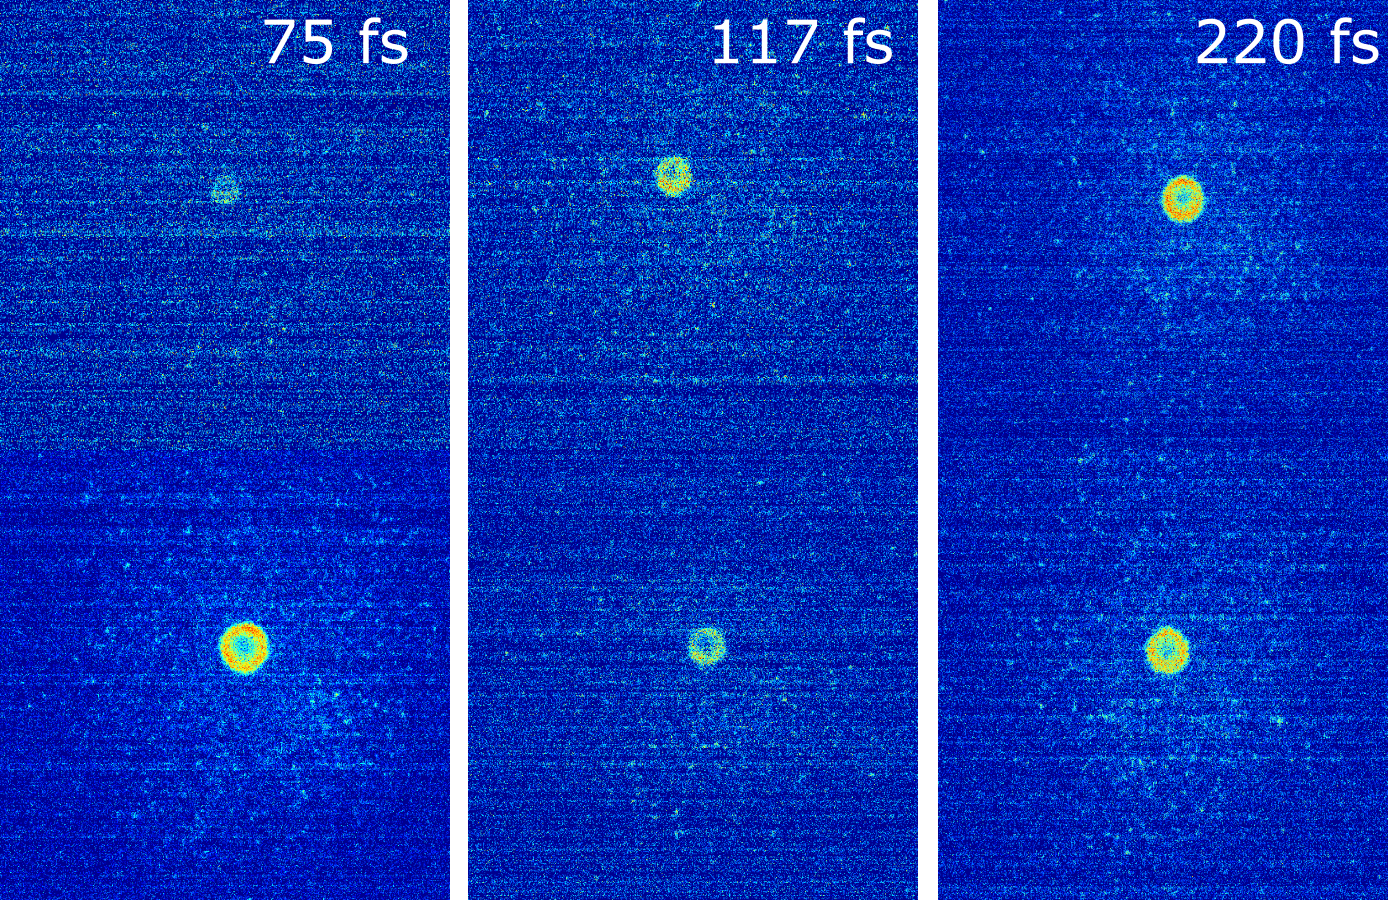
\includegraphics[width=0.5\textwidth]{../Images/results/MIR_He_pulsescan/raw/RAW_MIR_He_pulsescan.png}
\label{fig;MIrlaserraw}
\end{figure}

\subsubsection{Helium-Water Intensity Dependence}

Helium clusters at the same nozzle temperature $T_{nozzle}=11$ K and backing pressure of $P_{0}=30$ mbar, were doped with Water at a fix doping level $P_{dop}=1E-4$mbar pressure measured in the gas doping cell. At this nozzle temperature the Helium droplet have proximate $N=244647$ atoms before going trough the oven chamber and its doped with H$_{2}$O$_{dop}$=56 atoms. The VMI voltages were set to VMIx1 and the MCP and PHS to $1750$ V and $4000$ V respectively. The camera was stablish to exposure time of $t_{exp}=34 \mu$s. 100000 pictures were taken for 6 different laser power, at $2, 4, 6, 7, 8$ and $9.5$ W, measured before the laser beam enters to the detection chamber and its back focus by the mirror. 


\begin{figure}[h!]
\centering
\begin{subfigure}[l]{0.49\textwidth}
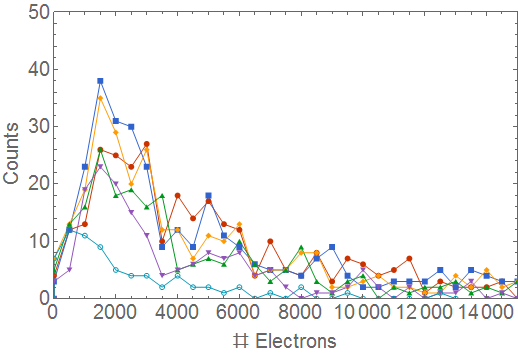
\includegraphics[width=1\textwidth]{../Images/results/MIR_He_waterIntensityscan/Helect.png} 
\end{subfigure}
\begin{subfigure}[l]{0.49\textwidth}
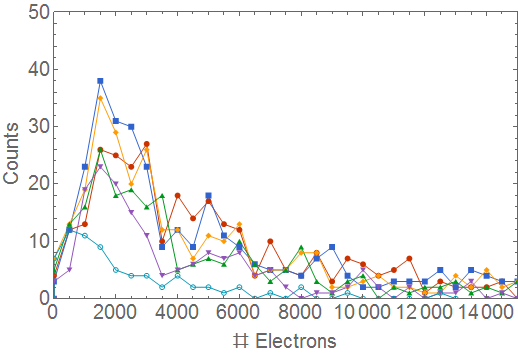
\includegraphics[width=1\textwidth]{../Images/results/MIR_He_waterIntensityscan/Helect.png}   				\end{subfigure}
\caption[MIR He-intensity dependence. Histogram]{On The left, the histogram for the Number of electrons for all intensity levels. On the right, the histogram for the max energies. The electron histogram was binned every 1000 e- while the energy was binned every 0.015 eV. The dashed line in the energy histogram shows the minimum energy that the lob finder algorithm can achieve.}
\label{fig:intehisto}
\end{figure}
 
Having the laser power, the intensity can be calculated for each laser power using the Xe cut off calibration. The legends in Fig.\ref{fig:intehisto} are the different laser intensities calculated for each of the laser power using Eq 3.2. On the right, the energy histogram have a clear distribution, there exist a predominant range of energies where for all intensities most of the electrons reach a max energy around 0.1  Furthermore, on the left histogram, most of the data is distributes in the peak near to 2000 e-, having a stiff rise from zero to 1000 e- and a slower decrease after 4000 e-, the counts for bigger electronic clouds  decrease for low intensities. Ass seen the blue and red line share a similar trend compared with high counts and a clear peak compared to the light blue and purple that have a broader distribution with lower counts.

\begin{figure}[h!]
\centering
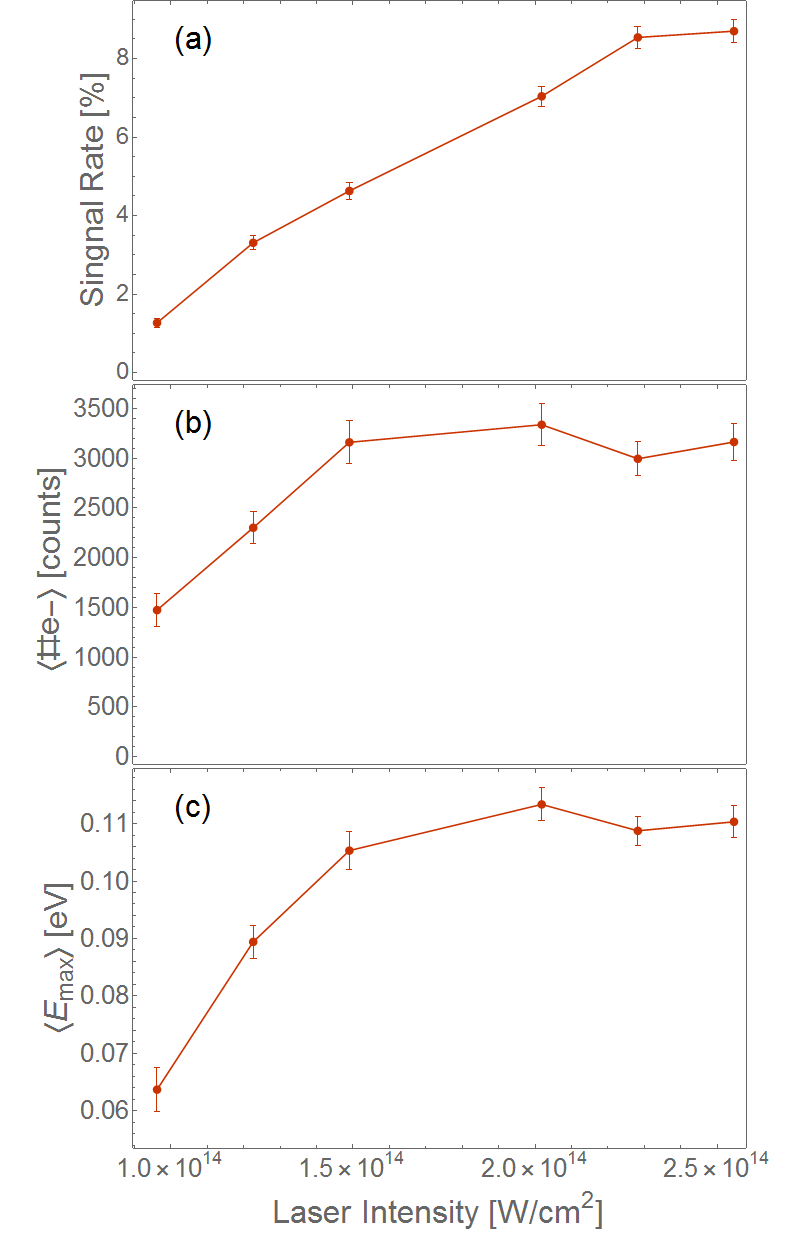
\includegraphics[width=0.5\textwidth]{../Images/results/MIR_He_waterIntensityscan/alltogether.png}
\caption[MIR He intensity dependence]{From top to bottom, signal rate and mean values of number of electrons ans max energy for different laser intensities}
\label{fig:Heintensimean}
\end{figure}

Fig \ref{fig:Heintensimean} top, shows the signal rate where a linear dependence is present for the laser intensity, meaning it  plays a fundamental role in the ignition of the process. At lower intensity, less probable to find signal and the highest intensity shows up to 4 time more signals than the lower one. At the same time we can identify that once the intensity reach $2E14$w/cm$^{2}$ the process starts to keep in a constant rate, it suggest the existence of  an intensity threshold, so the plasma formation will not be affected by the extra intensity radiated. This could be attribute to the ionization process, as known, minimum energy is needed ionized the dopant, but once these intensity is reach, all dopant will be completely ionized, so there is no longer energy transfer. 
On the bottom, the corresponding Mean of energy and number of electrons for each data set at it corresponding intensities. The mean values of $\#$e- and E$_{max}$, shows a  similar  disposition as the signal rate, the more intense the laser pulse the more energy and electrons can be found. The means values start to rise in a fast way on left but once it reach the 3 best intensities the divergence decrease and changes are less noticeable, following our previous assumption with the signal rate.

 
\subsubsection{Helium Pulse Duration Dependence}
 
In this data set, we present the result for the energy distribution of helium cluster doped with Xenon in different pulse duration.  Helium clusters at the same nozzle temperature $T_{nozzle}=10.5$ K and  backing pressure of $P_{0}=30$ mbar, were doped with Xenon at a fix doping level $P_{dop}=2.4E-4$ mbar pressure measured in the gas doping cell. At this nozzle temperature the Helium forms big clusters, with approximated $N=3150000$ atoms before going through the oven chamber and its doped with Xe$_{dop}$=75 atoms. The VMI voltages were set to VMIx1 and the MCP and PHS to $1600$V and $4000$V respectively. The camera was stablish to a exposure time of $t_{exp}=34 \mu$s. A first averaged mode signal was taken as a guide to the eye and after 100000 pictures were taken at 4 different pulse duration, at $65, 120, 200$ and $250$  fs, measured by the ELI-laser personal supporting us in the experiment, using FROG technique.
In the beginning of the experiment, we notice that the laser pulse have a dependence with the laser power,  longer pulses results in a weaker power. Table \ref{tab:pulsepower} resume the laser power obtained for each of the pulse duration. Fortunately the intensities didn't defer much and the intensities obtained are farther that the threshold to start the coulomb explosion as seen in the intensity scan above.
  
   
\begin{table}[]
\centering
\label{tab:pulsepower}
\begin{tabular}{|l|l|c|}
\hline
Pulse duration {[}fs{]} & \multicolumn{1}{c|}{Power{[}mW{]}} & Laser intensity {[}W/Cm\textasciicircum{}\{2\}{]} \\ \hline
65 & 8.8 & 1.5E14 \\ \hline
120 & 9.7 & 8E13 \\ \hline
200 & 9.8 & 5E13 \\ \hline
250 & 9.2 & 3.9E13 \\ \hline
\end{tabular}
\end{table}


\begin{figure}[h!]
\centering
\begin{subfigure}[l]{0.49\textwidth}
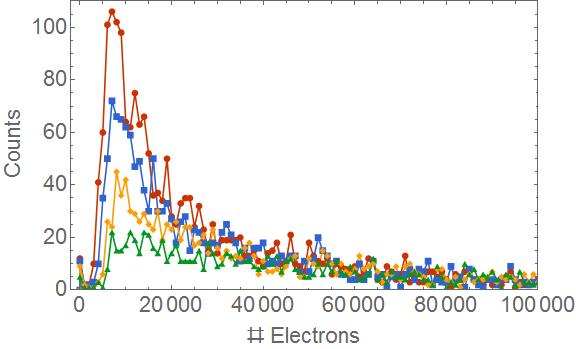
\includegraphics[width=1\textwidth]{../Images/results/MIR_He_pulsescan/raw/histoElec.png} 
\end{subfigure}
\begin{subfigure}[l]{0.49\textwidth}
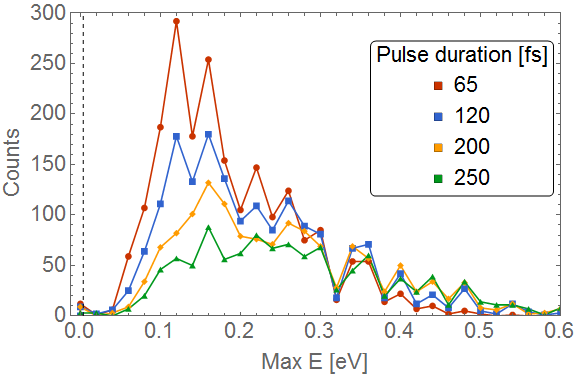
\includegraphics[width=1\textwidth]{../Images/results/MIR_He_pulsescan/raw/histoEnergc.png}   				\end{subfigure}
\caption[MIR He-intensity dependence. Histogram]{On The left, the histogram for the Number of electrons for all intensity levels binned every 1000 e-. On the right, the histogram for the max energies binned every 0.02 eV. The dashed line in the energy histogram shows the minimum energy that the blob finder algorithm can achieve.}
\label{fig:intehisto}
\end{figure}


Fig \ref{fig:intehisto} presents the histogram a for the number of electron and e max energy. The histograms shows a clear peak for the shorter duration while in the longest the distribution get broader. It means, that the smaller droplets are easily ignited on the shorter pulses, so we see the peak close to 100000 electrons, Furthermore, the energy histogram also  have a similar behaivour with a stiff peak that shifts around 0.15 to 0.2 eV depending on the pulse duration and with a slow decrease after 0.3 eV for all of them. The electron histogram on contrasts, does not present the peak shift but it does broaden its distribution with the pulse length.


% At the same time, on the energy distribution plot an interesting results are exhibited.  As usual all point represent the $\#$e- and E$_{max}$ of a single picture and the dashed line is the corresponding fit for each laser pulse following Eq. 3.12, letting the exponent and B-factor variable. In general all  plasmas behave in similar way, the fit lines goes almost parallel to each other and display the same B-factor  of 0.000179 that leads to a Radius for the electronic cloud of almost 500 $\mu$m with a factor of $2/5$. This similarity in the B-factor could represent that the energy distribution actually doesn’t seen affected by the laser pulse duration.
\begin{figure}[hbtp]
\centering
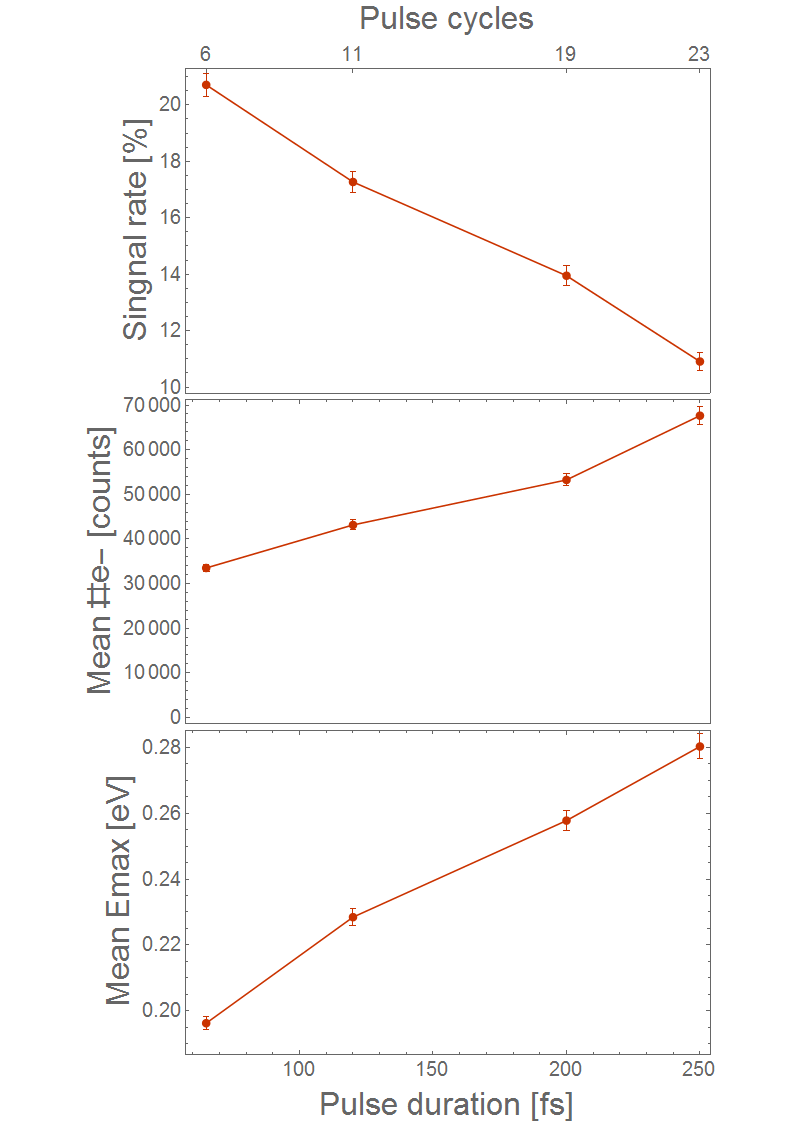
\includegraphics[width=0.5\textwidth]{../Images/results/MIR_He_pulsescan/raw/Alltogether.png}
\caption[MIR He pulse scan. Signal rate and mean values]{On the top, signal rate for the He-Xe  pulse duration scan. On the center and bottom,mean values for the $\#$e- an max energy depending on the laser pulse.}
\label{fig:Hepulseall}
\end{figure}

Fig. \ref{fig:Hepulseall} top, presents the signal rate for all the different pulses. As shown, the signal rate have a mark dependence on the  pulse duration, at the short pulses it have a ratio of almost 20$\%$  and it starts decreasing constantly  down to  10$\%$ at the longest pulse.  This behaviour is expected because, as saw in the intensity dependence, once we stretch the pulse the energy gets redistributed, so the laser field interacting in the ionization process is weaker, hence, the coulomb explosion ignition probability decrease. On the center and bottom, we plot the mean number of electrons and E$_{max}$  with dependency on the pulse duration. On contrast, the longer pulses are more likely to explode the bigger droplets. This also can be seen in the mean energies where the values rises with the pulse, also in the number of electrons. This result is surprising, especially if we compare it with the Intensity dependence mean values. Although, it is a non-intuitive results, it can be explained if we take into account that for longer pulses we have more cycles in the pulse. In consequence, even the initial ionization probability is lower for the first cycles, the electrons created on them will have more time to interact with the laser field, acquiring more energy and incrementing the electronic cascade that will start the coulomb explosion.


\section{Neon Nanoplasma in Mid-Infrared}

In the next section we present the results for the second beam time at ELI-Alps where we examines the nanoplasma formation of Neon clusters in Mid-Infrared laser pulses. The laser for this experiment was the same system used in Helium droplets. Neon cluster were created via a supersonic expansion with a conical nozzle with aperture d=15 $\mu$m of diameter. In order to obtain different cluster sizes, we used several nozzle temperatures around 37 K to 42 K, with a constant backing pressure of 50 mbar. Neon 0.6 were used to assure the purity of the clusters and to avoid any nozzle clog. Neon was doped with xenon through the gas doping cell. We will present 3 different experiments; Neon clusters size, Laser Pulse duration scan and Xe doping dependence. The VMI voltages keeps the same rate and the MCP and PHS voltages will be specified in each section. The pressures in the detection chamber oscillated during the experiments around 6E-8 mbar with the chopper open (Cluster beam in).  

Neon cluster formation presents a technical challenge due its solidification curve, at this backing pressure, small changes on the nozzle temperature leads to solidification of the gas, so we need to be careful at temperatures lower than 37 K. Another difference between neon and helium, is that neon clusters after the supersonic expansion are in a solid state. to determine the cluster size we use the  famous Hagena scale based on the work of \textit{Karnbach et al}\cite{karnbach_clulu:_1993}. Despite the difference and changes in the parameters, we perform the experiments without further problems.

\begin{figure}[h!]
\hfill
\begin{subfigure}[l]{0.4\textwidth}
\caption{Typical VMI signal for big neon droplets at high doping}
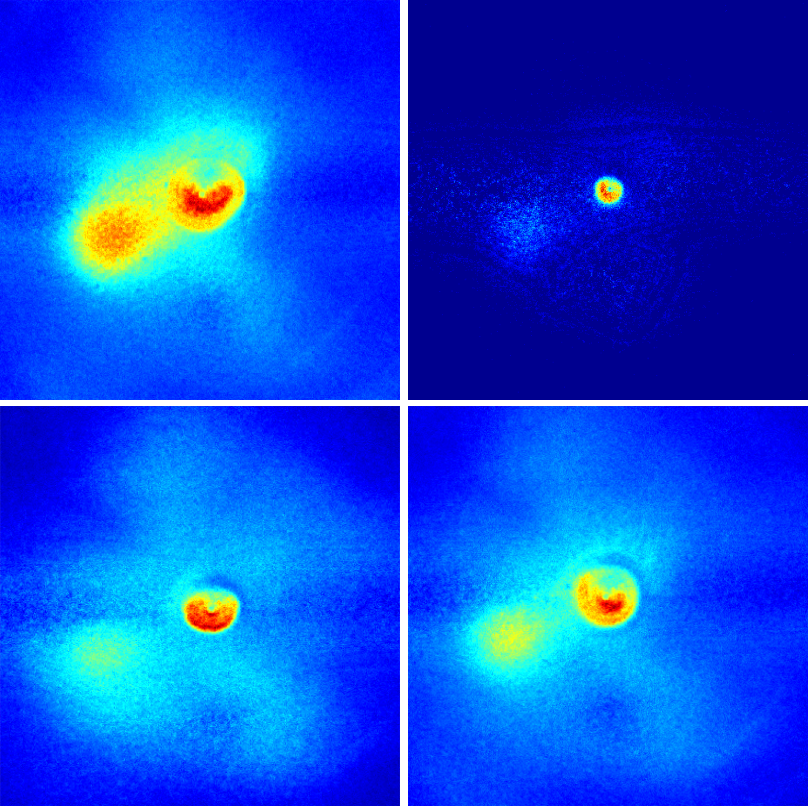
\includegraphics[width=1\textwidth]{../Images/results/MIR_Ne_XeDop_39K/RAw_NE_37KHighdop.png} 
\end{subfigure} 
\begin{subfigure}[l]{0.4\textwidth}
\caption{Typical VMI signal for big neon droplets at low doping}
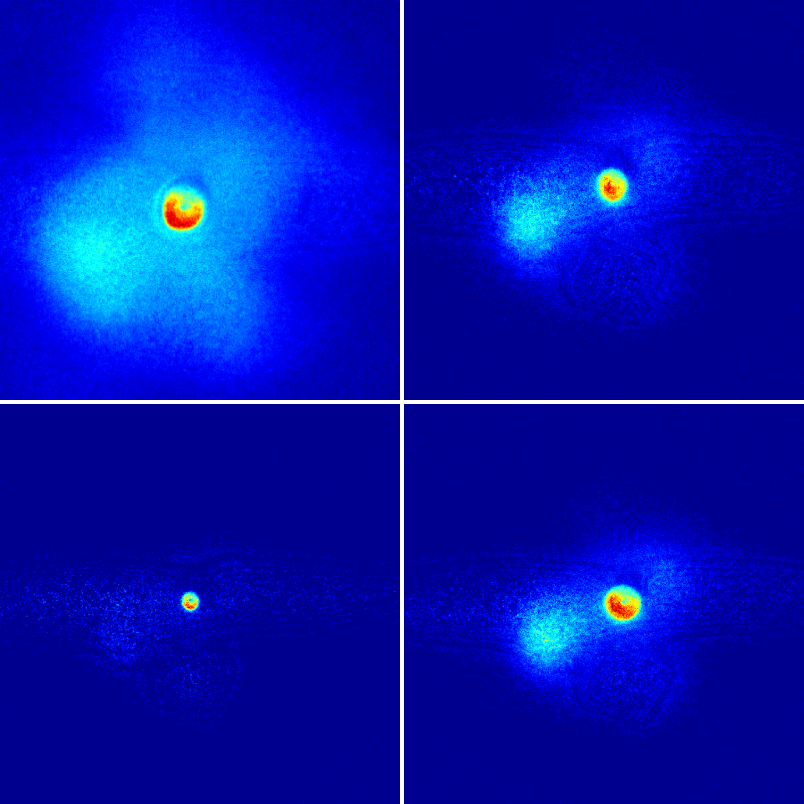
\includegraphics[width=1\textwidth]{../Images/results/MIR_Ne_XeDop_39K/RAw_NE_37Klowdop.png} 
\end{subfigure} \hfill


\hfill
\begin{subfigure}[l]{0.4\textwidth}
\caption{Typical VMI signal for small neon droplets at high doping}
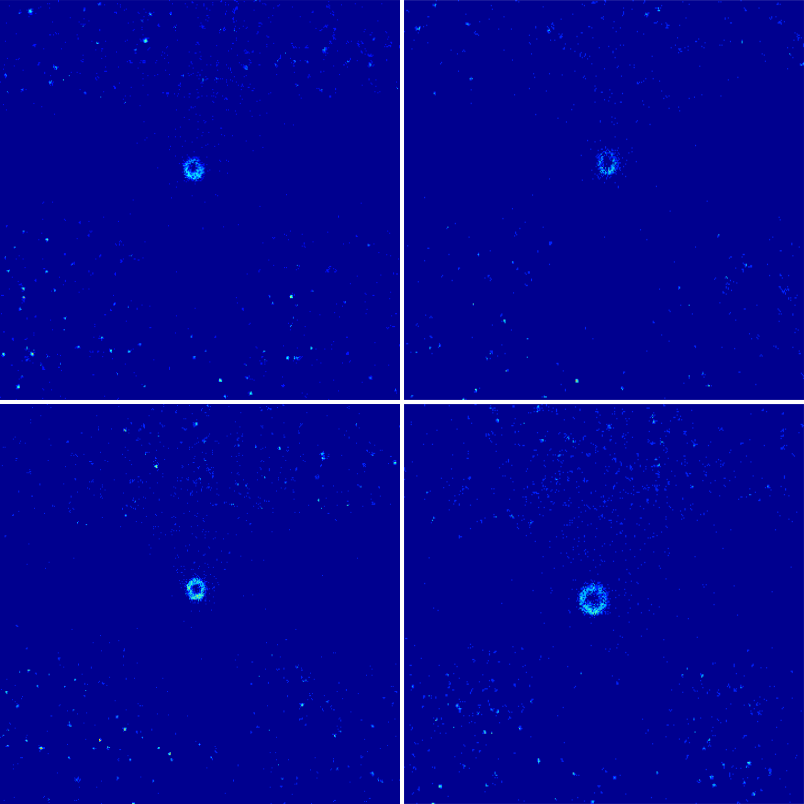
\includegraphics[width=1\textwidth]{../Images/results/MIR_Ne_XeDop_39K/RAw_NE_39KHighdop.png} 
\end{subfigure}
\begin{subfigure}[l]{0.4\textwidth}
\caption{Typical VMI signal for small neon droplets at low doping}
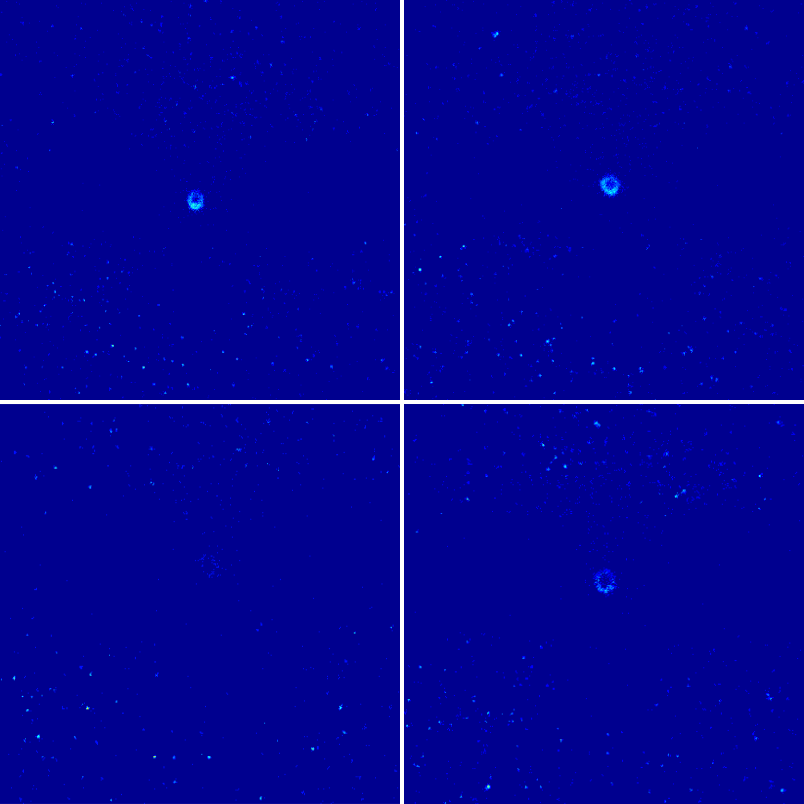
\includegraphics[width=1\textwidth]{../Images/results/MIR_Ne_XeDop_39K/RAw_NE_39Klowdop.png} 
\end{subfigure}
\hfill
\caption[MIR Neon raw samples]{Sample signals for the Neon nanoplasma for different sizes and doping levels. }
\label{fig:neonrwasample}
\end{figure}

Fig \ref{fig:neonrwasample} show a compilation of the raw VMI signals of neon plasma for different sizes and doping levels. In general all pictures have a similar distributions to the helium clusters. Fig. b, c and d represent a typical signal for doped neon clusters produced at temperatures over 39 K. The most common signals shapes are from small and medium size blobs with low intensity. additionally, there exist a small defect in the detector in the center-upper-right, where the brightness intensity decrease in all signal. It is cause because the large amount of electrons collected during the days burned the phosphor layer decreasing its detection efficiency, leaving a blind spot. Fortunately it is a systematic error and for future experiments we will just need to replace the screen. Additionally Fig  \ref{fig:neonrwasample} a, represents a typical signal of droplets at 37 K. These huge signals have  unusual shapes with elongations on the central blob and anisotropic high brightness that starts saturate the camera. Although, this signals was not a significant percentage of the results, they did appear regularly. One explanation for its irregular outline is given if we assume big clusters with irregular shapes. As Neon clusters are solid, it is possible that the bigger clusters will not condensate uniformly and in consequence they will create anomalies on the signal. Another explanation could be because of the large density of electron in big nanoplasma, they start to interact and create an unusual signal. Subsequently, this big droplets will be analyzed independently. These huge signals will not be taken into account in the next sections but gives us an interesting landmark in the study of Ne plasma. Nevertheless, most of the pictures presents regular shapes and the same protocol used in the helium can be applied. 


\subsection{Doping Dependence }

In this experiment small Neon clusters where doped with Xenon at different doping levels. The Neon clusters were created at the same nozzle temperature $T_{nozzle}=39$ K and at a backing pressure of $P_{0}=50$ mbar. Xenon were introduce at 7 different pressures measured in the oven chamber. The VMI voltages were set to VMIx1 and the MCP and PHS to $1800$ V and $4000$ V respectively. The camera was stablish to an exposure time of $t_{exp}=34$ $\mu$s  and the laser power were set to an average power of 10 W.


\begin{figure}[h!]
\hfill
\begin{subfigure}[l]{0.48\textwidth}
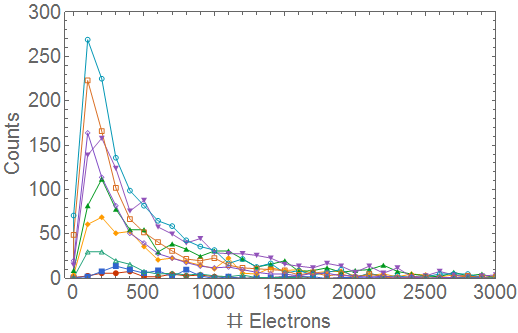
\includegraphics[width=1\textwidth]{../Images/results/MIR_Ne_XeDop_39K/HElec.png} 
\end{subfigure} 
\begin{subfigure}[l]{0.48\textwidth}
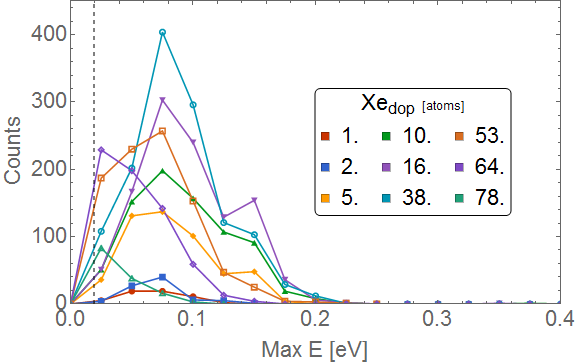
\includegraphics[width=1\textwidth]{../Images/results/MIR_Ne_XeDop_39K/HEnergc.png} 
\end{subfigure} \hfill

\caption[MIR Ne-Xe doping scan.Histograms]{On the left, The number of electron histograms for differnet Xe doping levels. On the right the energy histograms. The dashed line represents the minimun energy detected by the bloop finder algorithm.}
\label{fig:NeonXedophisto}
\end{figure}


Fig. \ref{fig:NeonXedophisto} shows the histogram for the number of electrons  and the Max energy. On the right, the histogram show a close distribution with shifting peaks from 0.05 to 0.1 eV and a drastic decrease up to 0.2 eV. The max counts increase regulary with the doping level until the purple line with Xe$_{202}$ and for higher doping the counts starts to reduce.. On the electrons histogram, a broader distribution is shown with a systematic peak at 3000 electrons, it means that the mean signal found, correspond to small clusters, even though  massive signals up to 30000 electrons can be found. 


\begin{figure}[hbtp]
\centering
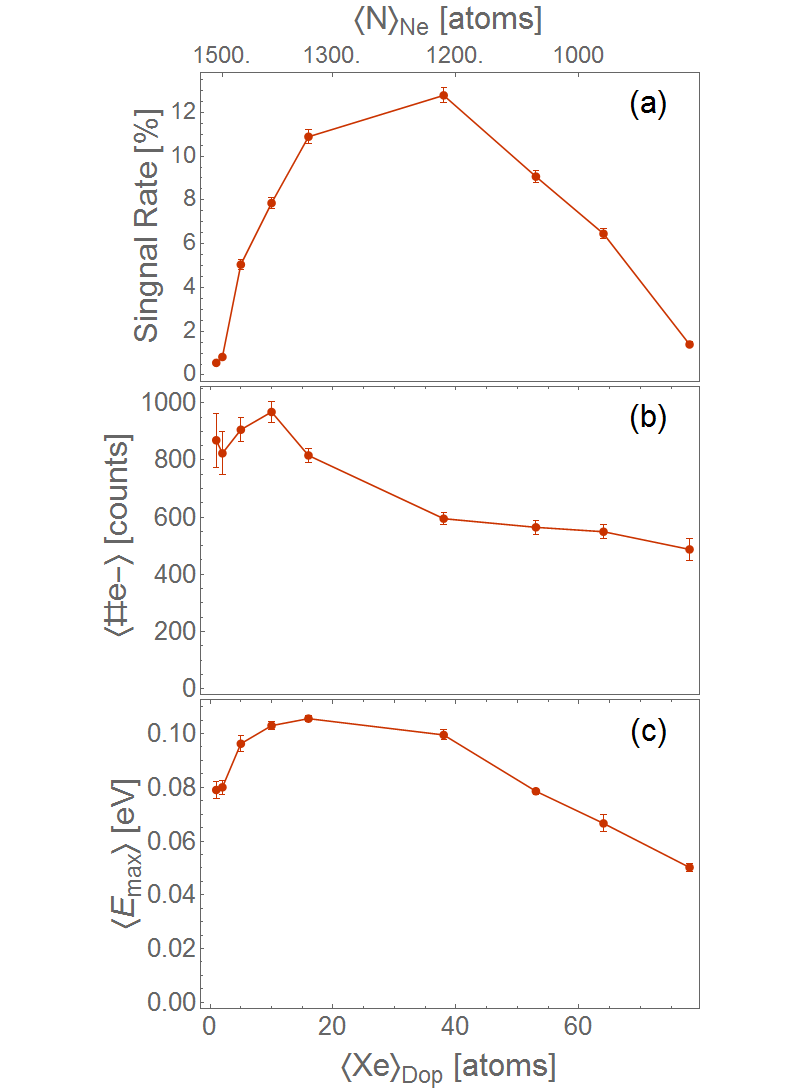
\includegraphics[width=0.5\textwidth]{../Images/results/MIR_Ne_XeDop_39K/Alltogether.png}
\caption[MIR Ne-Xe. Signal rate and mean values]{On the top, signal rate for the Ne-Xe doping dependence. On the center and bottom, the mean values for the $\#$e- and max energy depending on the laser pulse.}
\label{fig:NeXeall}
\end{figure}

Fig \ref{fig:NeXeall} top, shows the signal rate for the different pressures and the energy distribution for all doping levels. As notice on the left of the plot, the nanoplasma signal rate increase rapidly with the doping, until the best doping at 5E-5 mbar and keep constant for higher doping. This agrees to our previous results showing there exist a minimum doping level to have the most efficient plasma creation, and stronger doping does not help to have more signal. On contrary, for the highest doping levels we denote a small reduction in the signal rate showing that at this level, the clusters starts to be destroyed, and the signal rate goes down.
On one hand,  The mean values shows a constant increment in the energy for the first pressures, going in agreement with the signal rate, in other words, adding more dopant to the  Neon allows to achieve higher energies, but after reaching the doping limit pressure, a decrease in the mean energy appears. On the other hand, for the mean number of electrons, we see that for the first doping, the mean value keeps quite constants, but once we go upper the 5E-5 mbar, the mean decrease but the signal rate keeps high. This results shows that the doping increase the efficiency to ignite the nanoplasma, but at large doping level the mean value of electrons decrease, meaning that we are igniting small droplets. In short, is more efficient to ignite bigger droplets than small ones, because according to the data, the small ones need a larger amount of doping to be ignited while the large cluster just need a few atoms.

%
%For the Energy distribution, each colored point is the binning of the individual signal transformed to number of electrons and Energy, the dashed lines are the fits to the data according Eq 3.13 with $k$ and $B$ factor set free. As seen in the plot, the fit functions are quite similar to each other, sharing a comparable distribution. Table XXX shows the exponent, B-factor and the corresponding density and radius for the electronic cloud found from the fit. This functions agrees perfectly to or spherical cloud model, same as it happened on the NIR experiments. This relation proof that the Islam Model applied to the electron in a nanoplasma explosion could be accurate.

\subsection{cluster Size Dependence}

In order to understand the nano plasma explosion in Neon cluster, this experiment was done on different Neon cluster at a fix doping level with Xenon. The Neon clusters were created at 5 nozzle temperature 39, 40, 41, 42 and 44 K with a backing pressure of $P_{0}=50$ mbar. Xenon where introduce at a fix  pressures measured in the doping cell of 0.00036 mbar. The VMI voltages  where set to VMIx1  and the MCP and PHS to $1800$ V and $4100$ V respectively. The camera was stablish to exposure time of $t_{exp}=34$ $\mu$s   with the single shoot measurement scheme. The laser power were set to an average power of 11 W.

\begin{figure}[h!]
\hfill
\begin{subfigure}[l]{0.48\textwidth}
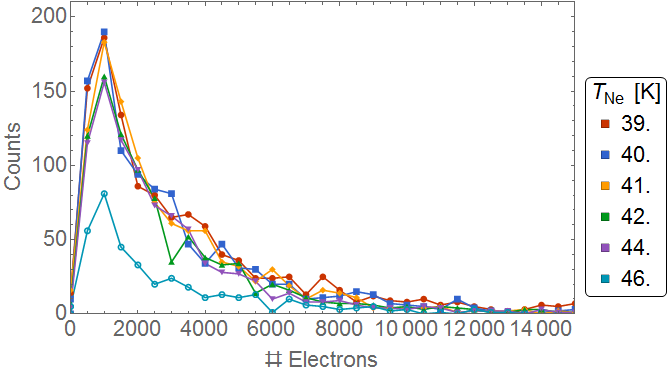
\includegraphics[width=1\textwidth]{../Images/results/MIR_Ne_DropletSize/HElec.png} 
\end{subfigure} 
\begin{subfigure}[l]{0.48\textwidth}
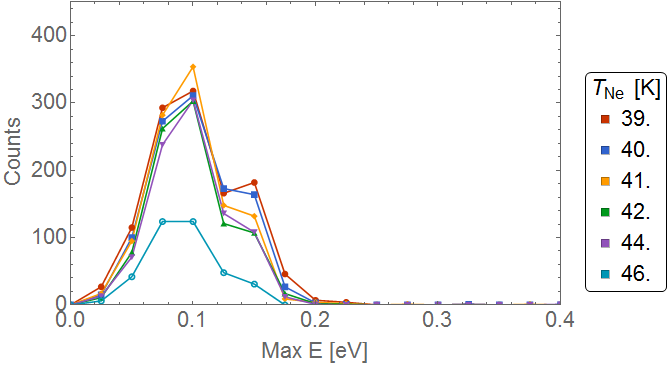
\includegraphics[width=1\textwidth]{../Images/results/MIR_Ne_DropletSize/HEnergc.png} 
\end{subfigure} \hfill
\caption[MIR Ne size dependence.Histograms]{From left to right, the number of electron histograms and the energy histograms for the different  number of atom <N> in the neon cluster. }
\label{fig:NeonsizeHisto}
\end{figure}

Fig. \ref{fig:NeonsizeHisto} shows the histogram for the number of electrons  and the max energy. On the right, the histogram have similar distribution independent of the cluster size, the biggest droplets present almost the same tendency just varying the peak count centred on 0.1 eV. On contrast, the light blue line is the only cluster size with a signification count change. Furthermore, on the left, the electron count histograms present similar trends with a peak around 1000 electrons, analogous to the histogram in the He-Xe doping. The counts just decrease due the signal rate as show in Fig \ref{fig:Nesizeall}, and slightly difference in the broaden at  bigger droplets. 

\begin{figure}[hbtp]
\centering
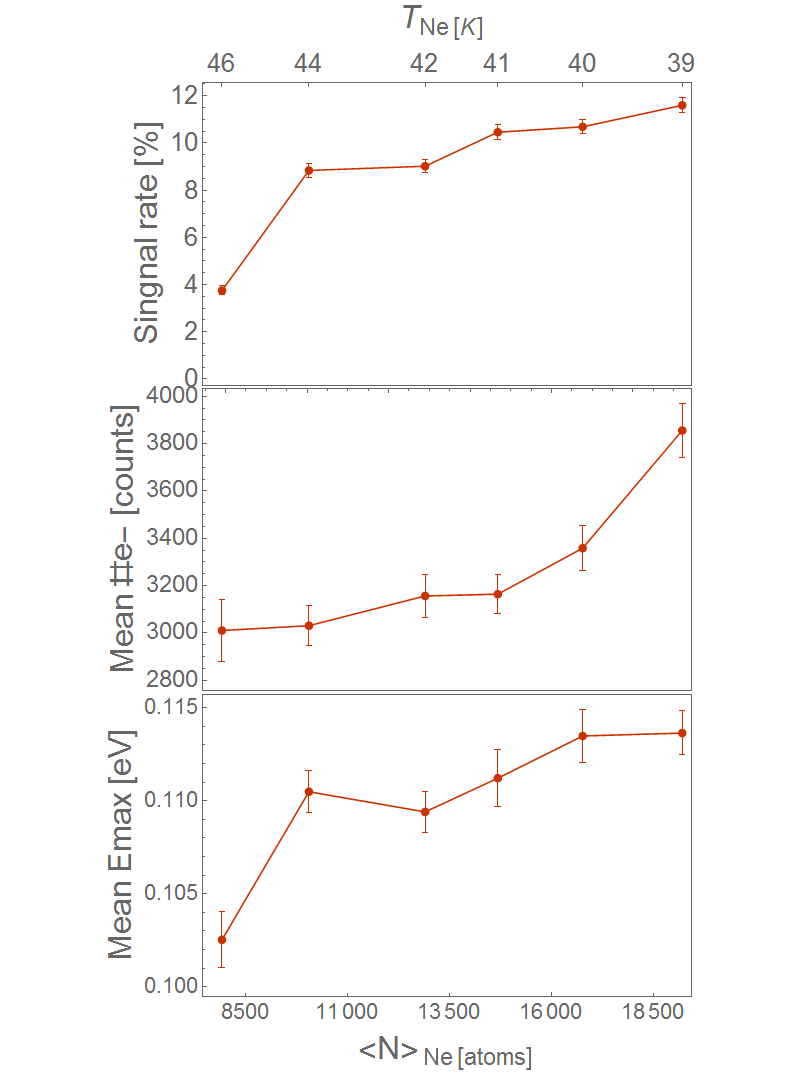
\includegraphics[width=0.5\textwidth]{../Images/results/MIR_Ne_DropletSize/alltogether.png}
\caption[MIR Ne size dependence. Signal rate and mean values]{On the top, signal rate for the Ne-Xe doping dependence. On the center and bottom, the mean values for the $\#$e- and max energy depending on the number of atoms <N> in the neon cluster.}
\label{fig:Nesizeall}
\end{figure}

Fig \ref{fig:Nesizeall} shows the signal rate and the energy distribution for the different nozzle temperatures. On the left, the signal rate shows an expected result where the bigger droplets present the higher rates and it decrease with the cluster size (high temperatures). The mean values show in Fig. \ref{fig:Nesizeall} center and bottom, have a trivial behaviour, congruent to the signal rate, both, mean number of electrons and Max energy, show an increase   with the cluster size. Again as in the He size dependence, the bigger droplets have more electrons to be detected so this relation is expected.

% For the Energy distribution there is no surprise neither, the data point and signal presents the same energy distribution as shown in the doping scan, The fit function was once again done based on Eq. 3.13 and give a exponent of $2/3$ following the spherical model. For the B factor, was in average $B=0.09$ given a density of 62 $\mu$m$^{-3}$ and a electronic cloud radius of 7 $\mu$m.
%
%The reason for this tendency is not clear, but if we assume the interaction dopant-cluster, small cluster could have a high probability of losing the ionized electrons in the beginning of the pulse, so the ignition process is less efficient, while for the bigger clusters, the ionized electron have more atoms to interact, so the losses are less, and in consequence the bigger clusters are more efficient to create the nanoplasma.


\subsection{Neon Pulse Duration Dependence}

The last measurement done in ELI-Alps was a laser pulse duration dependence. Neon cluster at a fix doping level with Xenon at a  nozzle temperature 39 K and a backing pressure of $P_{0}=50$ mbar  were shoot by the MIR laser pulse at 5 different pulse duration of, 48, 55, 64 71, and 94 fs. Xenon were introduce at a fix pressures measured in the doping cell at 0.0002 mbar. The VMI voltages were set to VMIx1 and the MCP and PHS to $1700$ V and $4000$ V respectively. The camera was stablish to exposure time of 34 $\mu$s with the single shoot measurement scheme. As in section 4.2.5 the pulse duration have a recurrent effect in the laser power, Table \ref{tab:Neonpulsepower} shows the different powers and consecutive the laser intensities at each data set was taken.

\begin{table}[t]
\centering

\begin{tabular}{|l|l|c|}
\hline
Pulse duration {[}fs{]} & \multicolumn{1}{c|}{Power{[}W{]}} & Laser intensity {[}W/Cm$^{2}${]} \\ \hline
48 & 10.5 & 2E14 \\ \hline
55 & 11 & 1.7E14 \\ \hline
64 & 11 & 1.5E14 \\ \hline
71 & 10.4 & 1.3E14 \\ \hline
94 & 8.6 & 1E14 \\ \hline
\end{tabular}
\caption{Neon pulse scan  intensity table.}
\label{tab:Neonpulsepower}
\end{table}


\begin{figure}[h!]
\hfill
\begin{subfigure}[l]{0.48\textwidth}
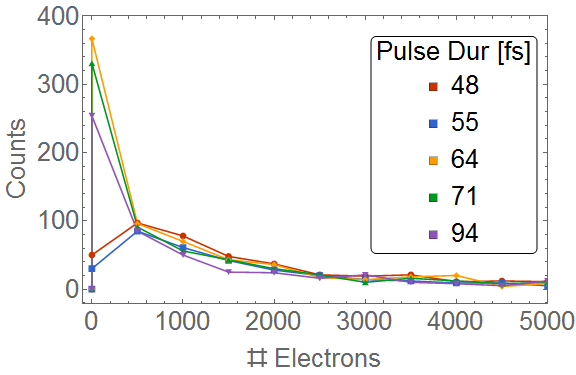
\includegraphics[width=1\textwidth]{../Images/results/MIR_Ne_pulseduration/HElec.png} 
\end{subfigure} 
\begin{subfigure}[l]{0.48\textwidth}
\includegraphics[width=1\textwidth]{../Images/results/MIR_Ne_pulseduration/HEnerg.png} 
\end{subfigure} \hfill
\caption[MIR Ne pulse duration. Histograms]{From left to right, the number of electron histograms and the energy histograms for the different laser pulse duration. The electron are binner every 1000 whiletle the energy histograms is binned every 0.02 eV }
\label{fig:NeonpulseHisto}
\end{figure}

Fig. \ref{fig:NeonpulseHisto} shows the histogram for the number of electrons  and the max energy. On the right, the histogram have diferentt distribution dependent of the cluster size. As seen, the longer pulser reach a broader range of energy in contrast to to the shorter pulses which have a clear and define peak centred at 0.1 eV. the initial positive slope is stiffer for the longer pulses who reach a first peak at 0.05 eV and decrease after 0.15 same as the shorter ones. Furthermore, on the left, the electron count histograms present a new trend with a peak distribution close to 0 e- for all pulses, what means that most of the signals have a extream low brightness and have a number of electrons lower that 1000.

\begin{figure}[hbtp]
\centering
\includegraphics[width=0.5\textwidth]{../Images/results/MIR_Ne_pulseduration/Alltogether.png}
\caption[MIR Ne pulse duration. Signal rate and mean values]{On the top, signal rate for the Ne-Xe doping dependence. On the center and bottom, the mean values for the $\#$e- and max energy depending on the pulse duration.}
\label{fig:Nepulseall}
\end{figure}

Fig. \ref{fig:Nepulseall} present the signal rate and mean values for the different pulse duration. Here the signal rates shows the same tendency that sec 4.2, The pulse duration plays an important role in the nanoplasma ignition, and the probability to create nanoplasma decrease constantly with the pulse, in this case, almost having no signal for pulses longer than 100 fs. Surprisingly in the mean values for the electron numbers and energy also shown a strong relation to the pulse duration. As table \ref{tab:Neonpulsepower} reefers, the intensity that the laser gave were almost the same, so the variations in the mean values confirm that at longer pulses the rates to ionize bigger droplets increase. So as shown, we can see the same effect regardless the cluster element and doping level. For understand this result we need to picture how the stretch of a pulse will derive in more cycles in it. The first cycles will be determinant for the Ionization of the dopant, the electrons create in the beginning of the pulse will have more time to interact with the laser field, and in consequence they will acquire more energy and time to interact with the cluster. Once we stretch the pulse, the electrons produced in this first cycle will see more cycles, and the ionization of the cluster will be more efficient. 






